\documentclass{jcgt}

\setciteauthor{Mikhail Letavin, ...}
\setcitetitle{FlexClip – the direct Bézier patch ray tracing revisited}
%\setheadtitle{Abbreviated title, only if full title won't fit in page headers}

% Mark submissions with the date of submission using the following line:
\submitted{\today}

% Once an article is accepted accepted, switch to the following line and comment the preceding one. The editor will supply the argument values.
\accepted{submitted}{accepted}{published}{Editor Name}{vol}{issue}{1}{1}{year}
\seturl{http://jcgt.org/published/vol/issue/num/}


%%%%%%%%%%%%%%%%%%%%%%%%%%%%%%%%%%%%%%%%%%%%%%%%%


\begin{document}

\title{FlexClip – the direct Bézier patch ray tracing revisited}

\author
       {Mikhail Letavin, ...
       }

\teaser{
\begin{table}[h!]
\resizebox{\textwidth}{!}{%
	\centering 
	\begin{tabular}{ *{6}{c} }
		%\hline		
		\begin{minipage}{.15\textwidth}
			\centering
			\includegraphics[width=\linewidth]{pic/teapot_Geo.png} \\
			\textbf{Utah teapot} \\ patches: 32
		\end{minipage}
		&
		\begin{minipage}{.15\textwidth}
			\centering
			\includegraphics[width=\linewidth]{pic/Skull_bot_frontGeo.png} \\
			\textbf{Skull bot} \\ patches: 6396
		\end{minipage}
		&
		\begin{minipage}{.15\textwidth}
			\centering
			\includegraphics[width=\linewidth]{pic/kircheGeo.png} \\
			\textbf{Kirche} \\ patches: 4481
		\end{minipage}
		&
		\begin{minipage}{.15\textwidth}
			\centering
			\includegraphics[width=\linewidth]{pic/pyramidGeo.png} \\
			\textbf{Pyramid} \\ patches: 614
		\end{minipage}
		&
		\begin{minipage}{.15\textwidth}
			\centering
			\includegraphics[width=\linewidth]{pic/sofaGeo.png} \\
			\textbf{Sofa} \\ patches: 666
		\end{minipage}
		&
		\begin{minipage}{.15\textwidth}
			\centering
			\includegraphics[width=\linewidth]{pic/sauele_allGeo.png} \\
			\textbf{Columns} \\ patches: 1904
		\end{minipage}
		\\
		\begin{minipage}{.15\textwidth}
			\centering
			\includegraphics[width=\linewidth]{pic/kitchenGeo.png} \\
			\textbf{Kitchen} \\ patches: 33497
		\end{minipage}
		&
		\begin{minipage}{.15\textwidth}
			\centering
			\includegraphics[width=\linewidth]{pic/bob5Geo.png} \\
			\textbf{Bob5} \\ patches: 85542
		\end{minipage}
		&
		\begin{minipage}{.15\textwidth}
			\centering
			\includegraphics[width=\linewidth]{pic/tahoro_frontGeo.png} \\
			\textbf{Tahoro} \\ patches: 172572
		\end{minipage}
		&
		\begin{minipage}{.15\textwidth}
			\centering
			\includegraphics[width=\linewidth]{pic/mascotangstGeo.png} \\
			\textbf{Mascotangst} \\ patches: 33724
		\end{minipage}
		&
		\begin{minipage}{.15\textwidth}
			\centering
			\includegraphics[width=\linewidth]{pic/helmetGeo.png} \\
			\textbf{Helmet} \\ patches: 6608
		\end{minipage}
		&
		\begin{minipage}{.15\textwidth}
			\centering
			\includegraphics[width=\linewidth]{pic/zeroGeo.png} \\
			\textbf{Zero} \\ patches: 100688
		\end{minipage}
	\end{tabular}}
	\caption{Test scenes}\label{tbl:test_scenes}
\end{table}
}

\maketitle
\thispagestyle{firstpagestyle}

\begin{abstract}
\small
This paper presents the FlexClip - a novel direct Bézier surface rendering algorithm based on a widely used Bézier clipping and its later interval-based modification - GeoClip. Novel modifications are aimed to overcome existing bottlenecks and further improve algorithm performance in application to  interactive Bézier patch rendering. The performance numbers comparison for scalar C++ and SIMD-optimized versions are provided, demonstrating the benefits of new method.
\end{abstract}


%-------------------------------------------------------------------------
\section{Introduction}
\label{sec:introduction}
With growing complexity of 3D film and animation projects, scene tessellation with its large memory requirements and need for complex acceleration structures increasingly becomes a bottleneck in a modern raytracing pipeline. A demand for performant and accurate algorithms for direct rendering of higher-order primitives used in CAD/CAM applications and/or physical simulation – such as NURBS, Catmull-Clark or implicit surfaces - becomes more and more relevant. In answer to such a demand, a growing number of direct rendering solutions appear in research. Probably one of the most active research topics in this area is a problem of bicubic Bézier patch rendering, since most of the primitives mentioned above can be represented by Bézier patches without sacrificing flexibility, accuracy and compactness.

\subsection{Related Work}
\label{sec:relatedwork}

\begin{figure}[th]
	\centering
	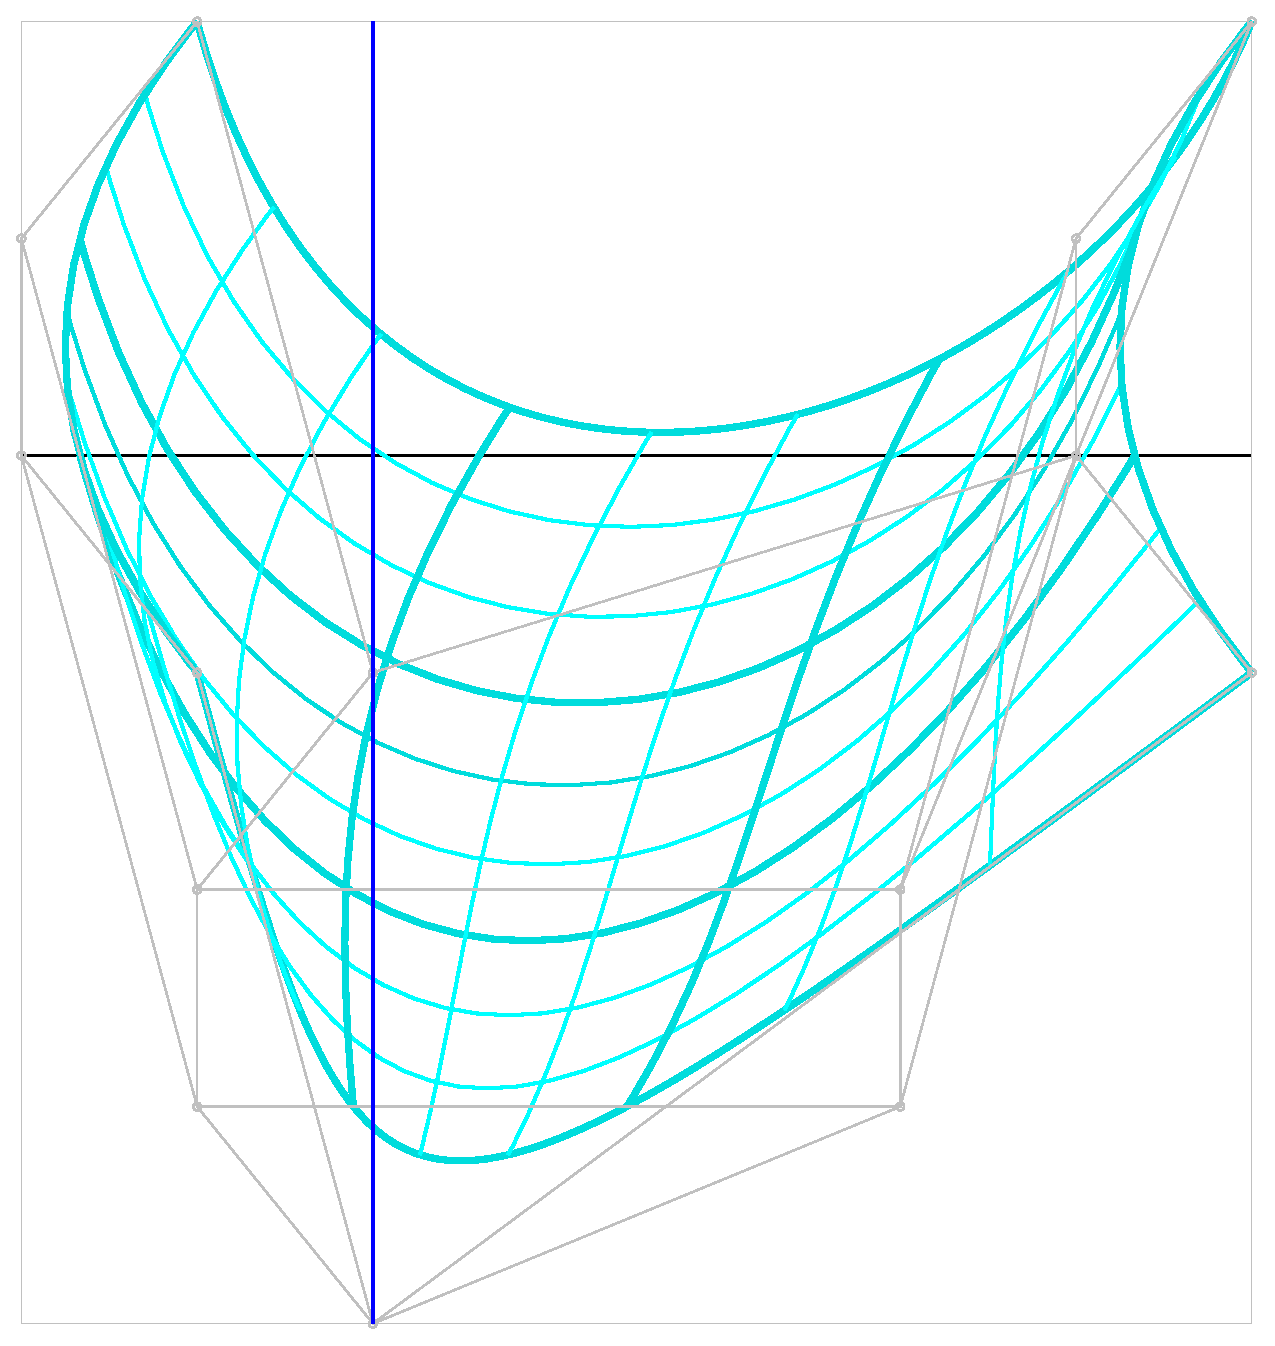
\includegraphics [ width=0.3\textwidth ]{pic/bclip1.eps}
	\hfill
	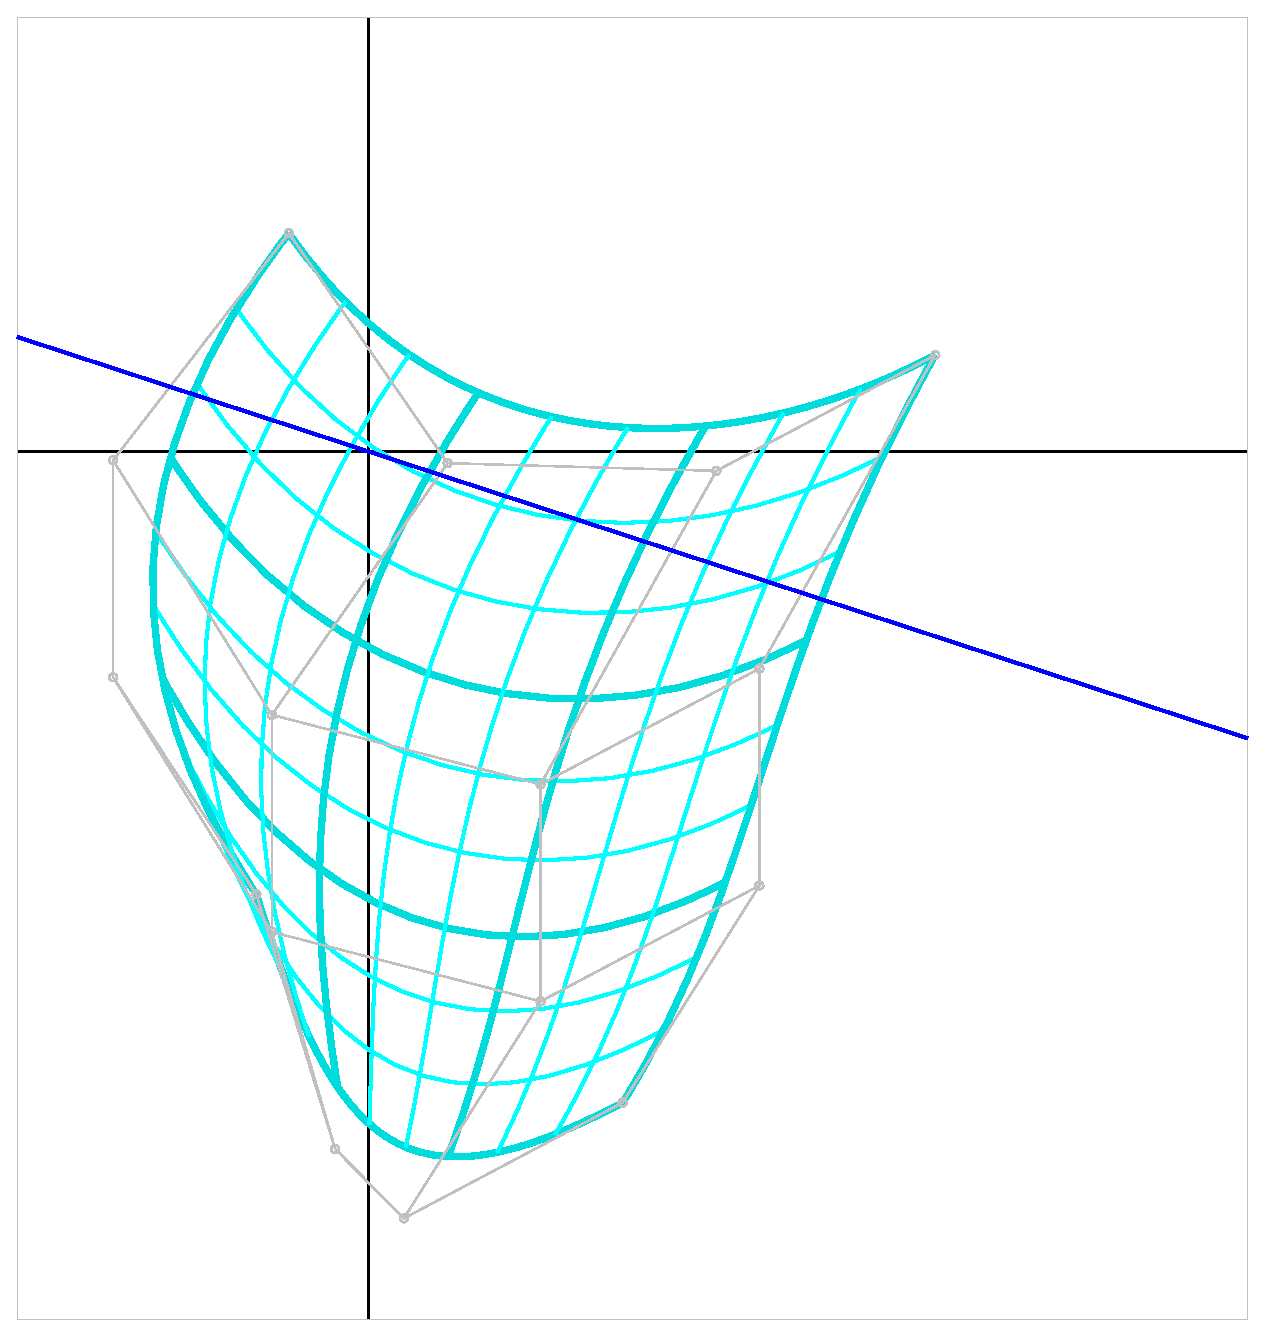
\includegraphics [ width=0.3\textwidth ]{pic/bclip3.eps}
	\hfill
	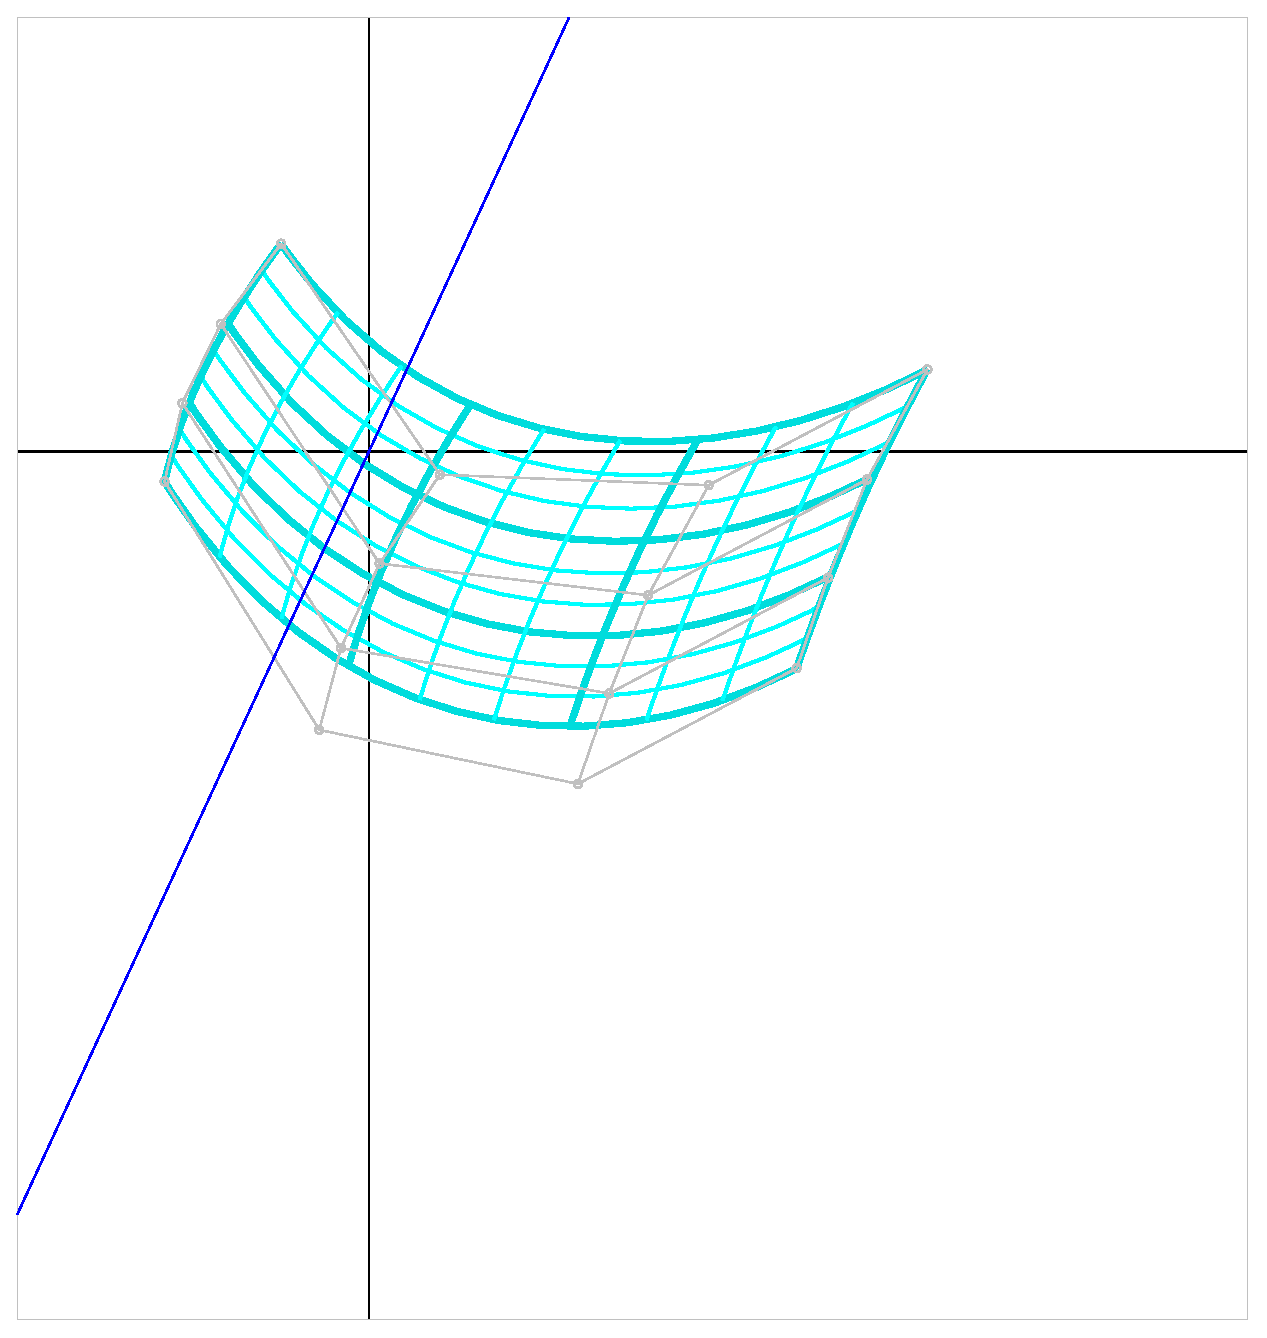
\includegraphics [ width=0.3\textwidth ]{pic/bclip5.eps}
	% \hfill
	% \includegraphics [ width=0.23\textwidth ]{pic/bclip7.eps}
	\\ % <-- Line break
	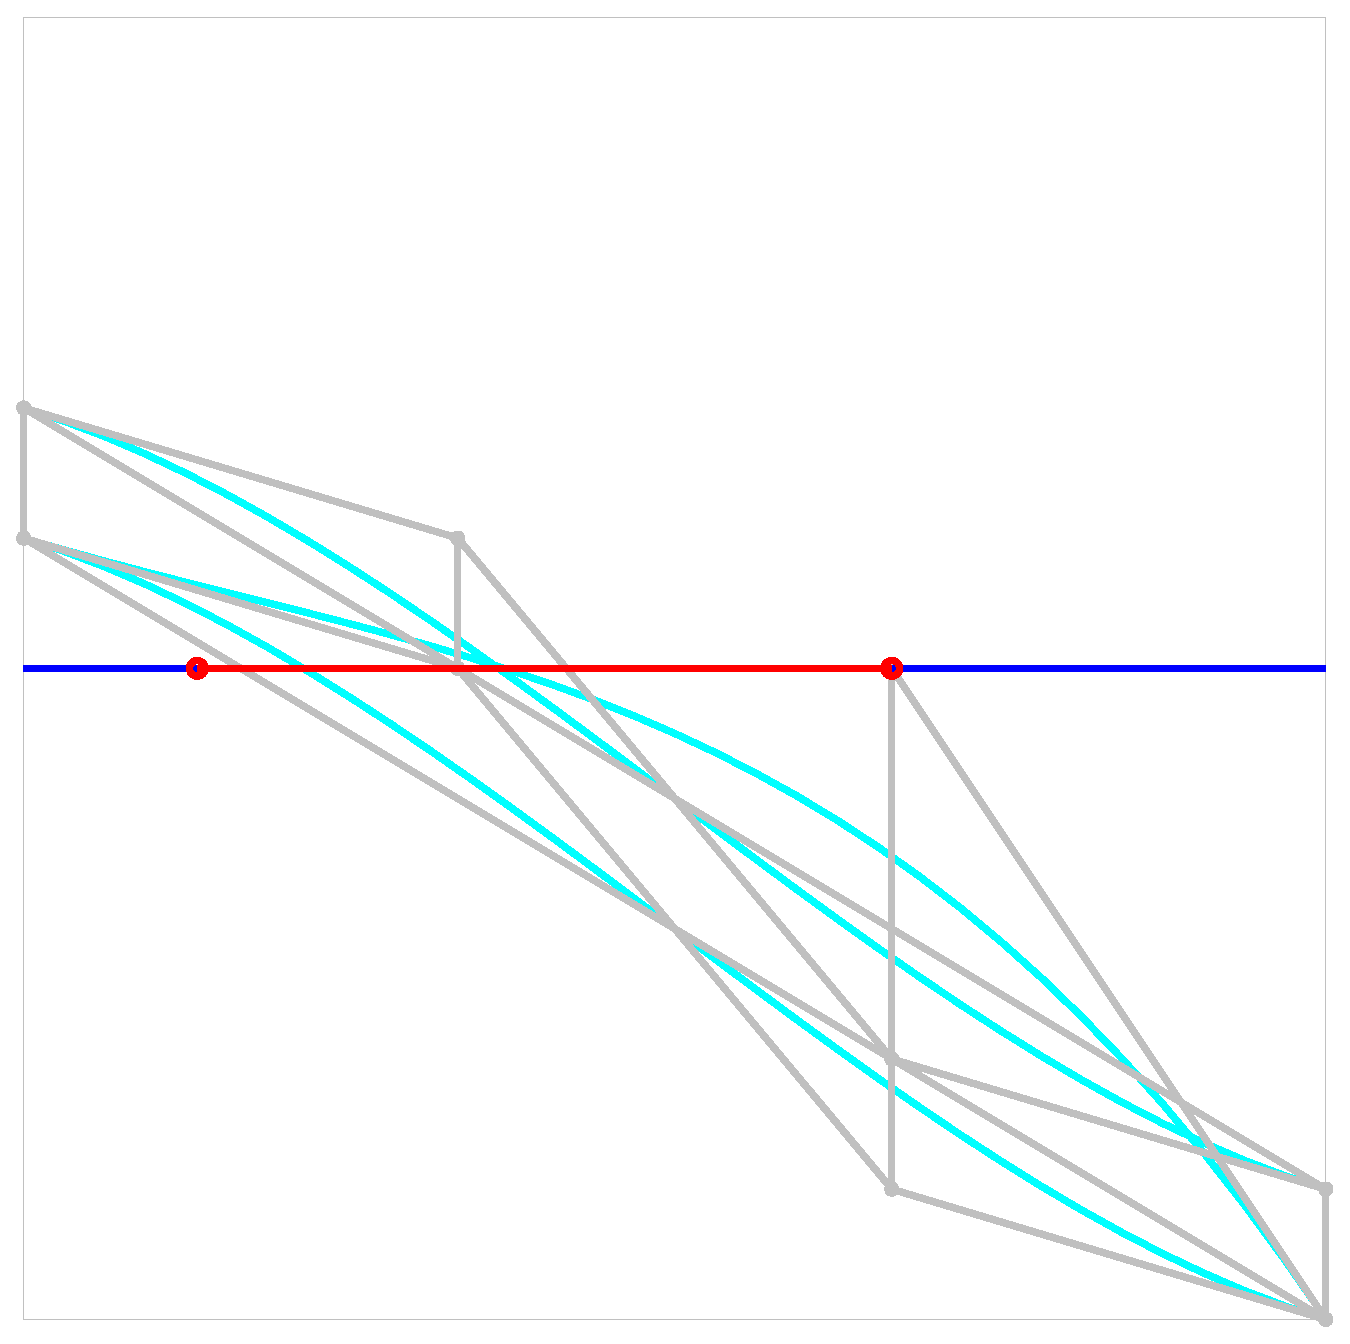
\includegraphics [ width=0.3\textwidth ]{pic/bclip2.eps}
	\hfill
	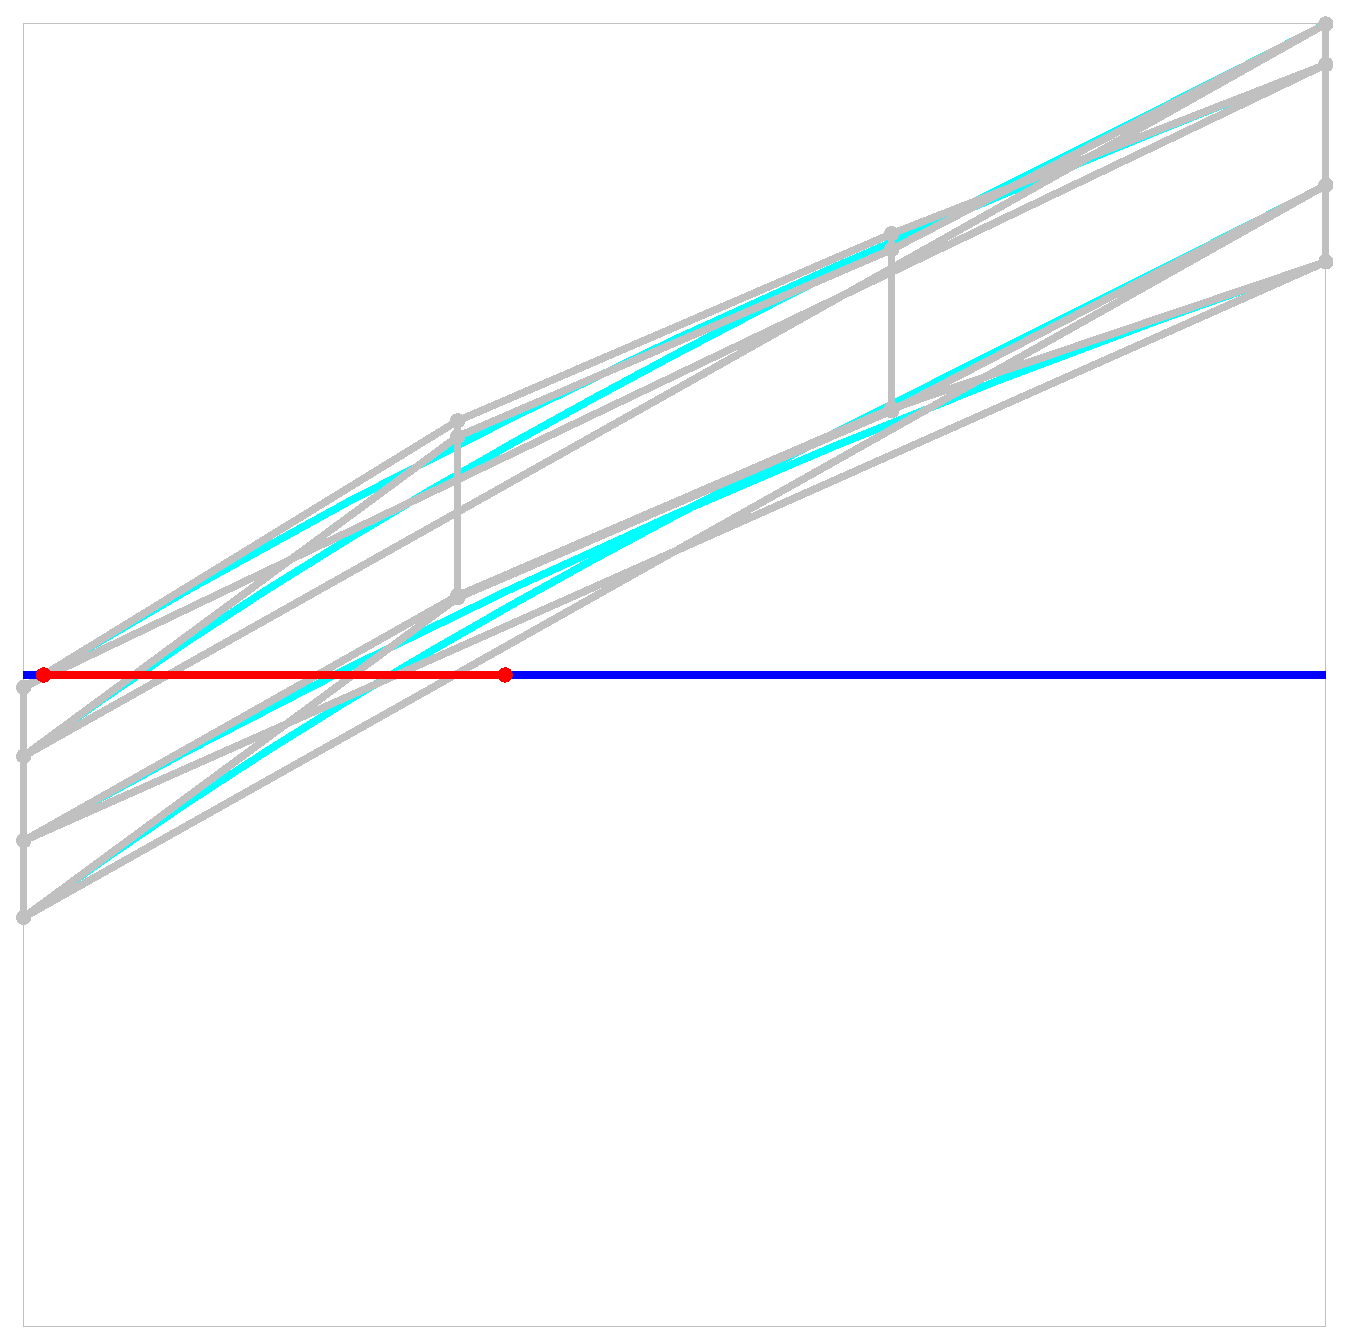
\includegraphics [ width=0.3\textwidth ]{pic/bclip4.eps}
	\hfill
	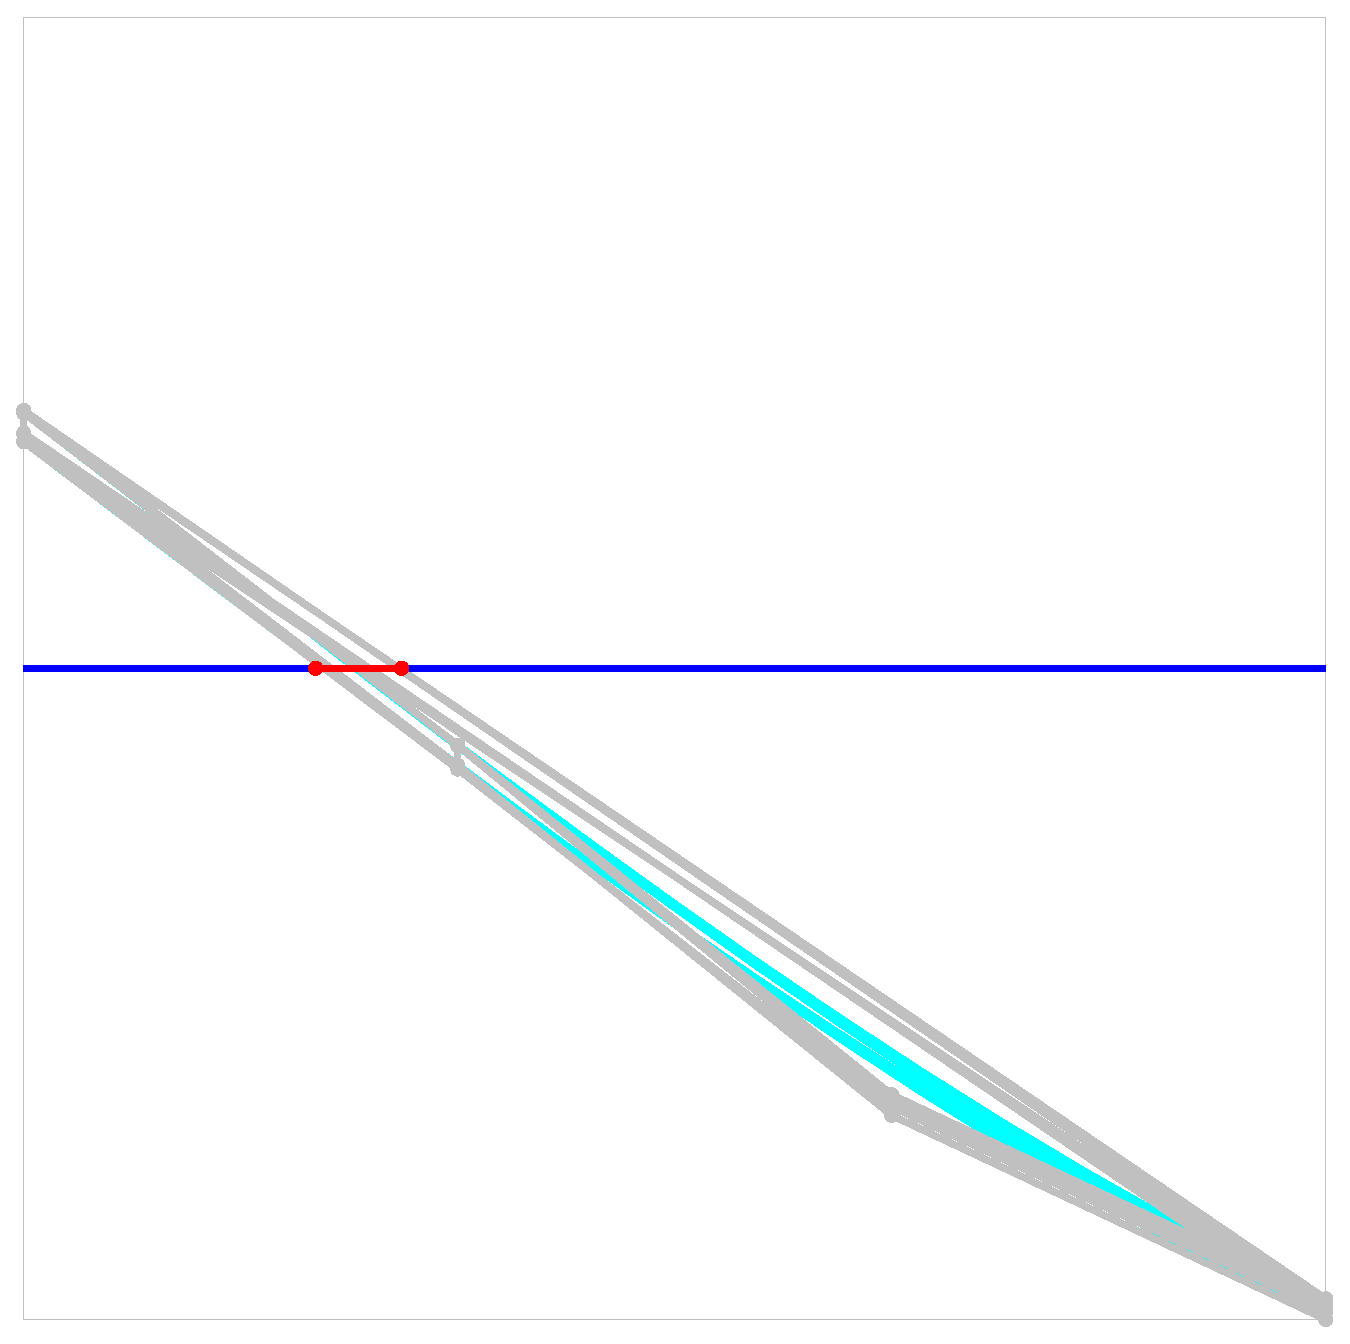
\includegraphics [ width=0.3\textwidth ]{pic/bclip6.eps}
	% \hfill
	% \includegraphics [ width=0.23\textwidth ]{pic/bclip8.eps}
	\caption{Initial iterations of the Bézier clipping. Following the original algorithm, the patch is first projected to the ray-centric 2D space, then line is chosen for each parameter, distances for the explicit patch are computed and clipping is performed in 1D iteratively. Consecutive iterations are interleaved in U and V parametric dimensions. The upper row shows patch clipping progress in 2D, and the lower one shows the explicit projected patch along with detected parameter ROI for every iteration }
	\label{fig:StartIter}
\end{figure}

Among the other direct parametric patch rendering algorithms, Bézier Clipping \cite{NISHITA90} since its initial publication, gained a reputation of robust and elegant rendering solution, which is free from limitations inherent to other approaches.

The basic idea of Bézier Clipping is, after projecting a Bézier surface to so called "explicit" (or "non-parametric") space, to identify a parametric region of interest (ROI) where ray/patch intersection is possible (using a convex hull property), then to clip away non-intersecting parts of the patch and repeat this process iteratively until either intersection threshold is passed, or miss is reported. Possible multiple intersections cases are detected by analyzing the resulting ROI size, and handled by subdividing the patch in half and processing the resulting subpatches one by one using a stack. Several initial algorithm steps are depicted on figure \ref{fig:StartIter}. The Bézier Clipping algorithm is described in detail in \cite{NISHITA90} and \cite{EFREMOV05}.

Operating this way, Bézier Clipping takes the best from both the fixed point iteration and subdivision algorithms – it enjoys the quadratic convergence rate\cite{SCHULZ09}, it is able to robustly find all the intersections, it doesn’t require any preliminary patch subdivision and doesn’t suffer from the initial guess problem like Newton-Raphson iteration method. 

However, Bézier Clipping is not an ideal solution. Due to its iterative nature, floating point accuracy and computational cost issues still remain not fully resolved, stimulating researchers to propose modifications and enhancements to this algorithm.

Several years later after original algorithm publication, \cite{CAMPAGNA97} identified a problem with false intersections reporting and proposed a way to mitigate it. \cite{EFREMOV05} proposed several stability and robustness modifications like a safe way to deal with multiple identical intersection points, moving termination criteria from parametric to projected 2D space and automatic view-dependent computation of termination threshold. \cite{Tejima2015subdivision} described a Bézier clipping implementation details focusing on the application to full-featured OpenSubdiv\cite{OpenSubdiv} Catmull-Clark surfaces approximation and rendering.

Several attempts have been made to improve upon the quadratic convergence rate of original algorithm and overcome its performance corner cases. The main idea behind those modifications is to drop the original piecewise-linear convex hull bounds during the ROI search, and to compute pairs of quadratic or cubic bounding curves instead. Bounding curve pairs yield analytically computed root pairs, which, in turn, can be used as new, tighter ROIs. \cite{BARTON2007125} proposed a degree reduction/elevation scheme for such quadratic bounds computation. \cite{LIU2009547} used the same approach for obtaining cubic bounds when dealing with higher-order curves. Other similar approaches exist, aimed to increase numerical robustness or provide tighter bounds, like \cite{WuLi22}.

Unfortunately, while demonstrating a super-quadratic convergence rate and being well suited for root finding and higher order curve/curve intersection, those algorithms are not directly applicable to the interactive patch rendering. This is due to somewhat complicated bounds calculations, which, in addition to quadratic solver, result in a significantly increased iteration cost compared to the original Bézier clipping. The notable exception here is North\cite{NORTH07}, who developed the GeoClip – an elegant geometry interval clipping algorithm based on hybrid curves, which uses a very simple and minimalistic approach to bounding curve computation.

This study uses North’s GeoClip\cite{NORTH07} and \cite{EFREMOV05} results as a base for an attempt to further improve the rendering algorithm performance and stability. Another purpose is to provide some important low level implementation details often omitted in original publications. We haven't investigated yet any theoretical algorithm details and haven't even touched any topics related to other domains of algorithm applicability, such as curve/curve intersection or root finding. Instead, we concentrated strictly on application to interactive patch rendering.


\section{Generic algorithm modifications}

The original Bézier Clipping is a well balanced algorithm. It was able to find an equilibrium between computational cost and effectiveness of every step. But still, some opportunities could be found to "squeeze a little air" from various parts of the implementation. This section describes improvements and important performance-affecting details that are applicable to both original Bézier Clipping and any of its derivatives, such as GeoClip. Unless stated below, the remaining algorithm details are inherited from the algorithm version by \cite{EFREMOV05}.

\begin{figure}[t!]
	\centering
	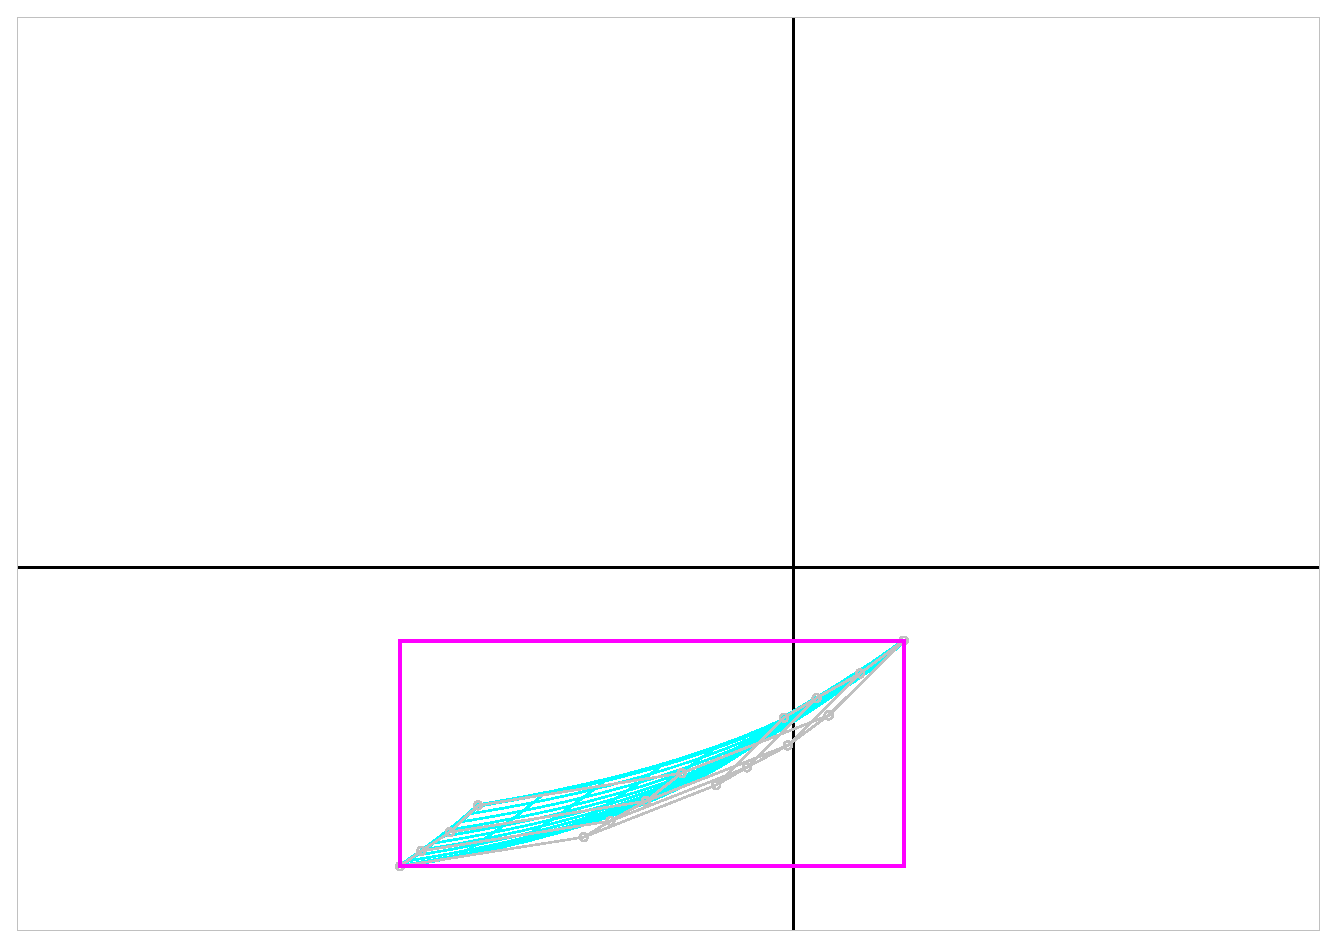
\includegraphics [ width=0.4\textwidth ]{pic/bclip19.eps}
	%\hfill
	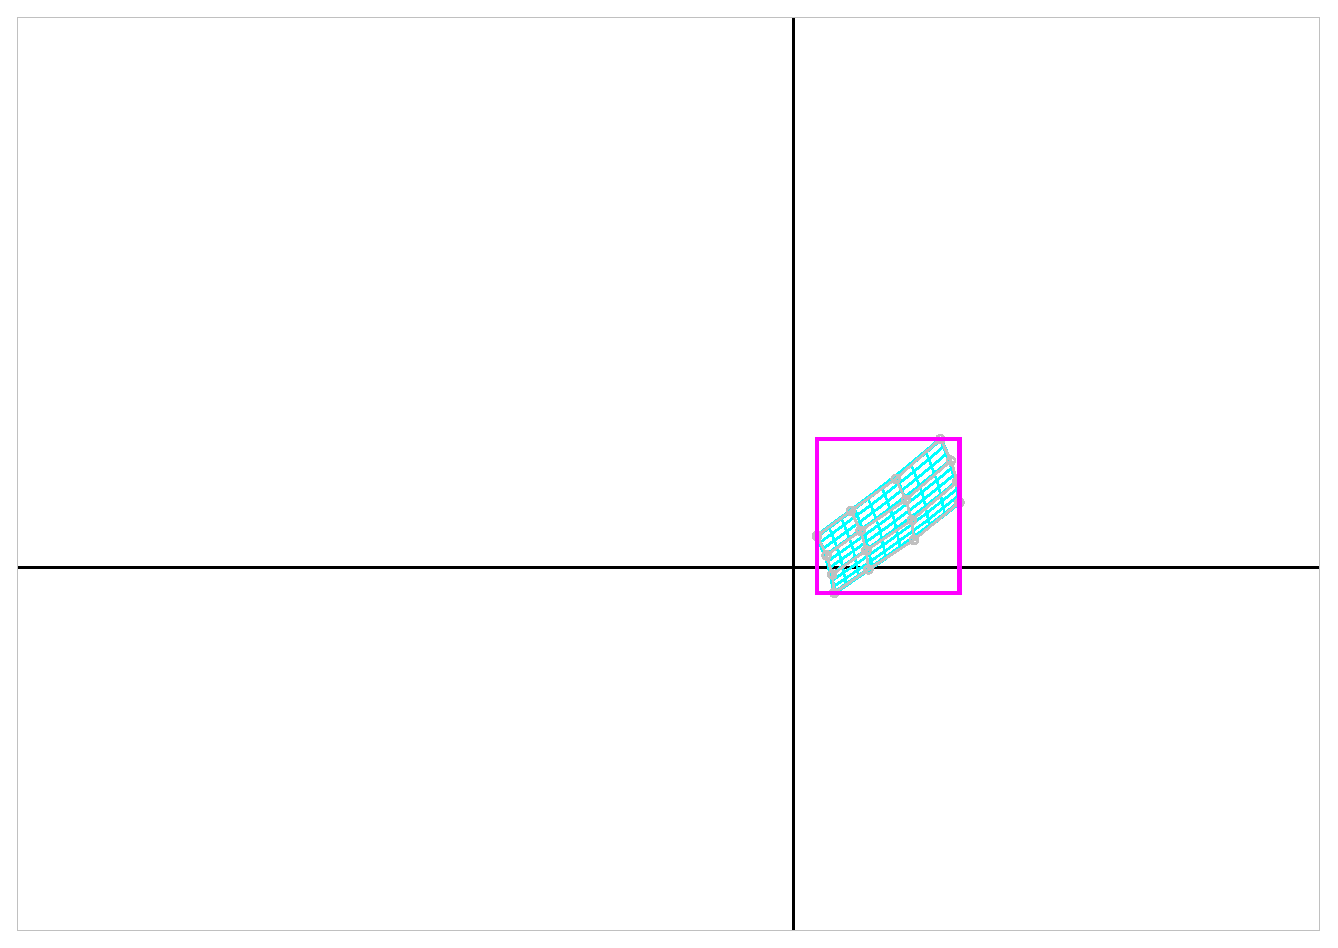
\includegraphics [ width=0.4\textwidth ]{pic/bclip22.eps}
	%\hfill
	%\includegraphics [ width=0.3\textwidth ]{pic/bclip29.eps}
	\caption{Cases when bounding box test reports a miss, saving further iterations}
	\label{fig:bbox_test}
\end{figure}

\subsection{2D bounding box miss test and new termination criteria}
According to our experiments, it is highly beneficial to perform a 2D bounding box check right after every clipping iteration and every sub-patch stack pop. This simple test consists of the clipped 2D patch bounding box computation from freshly obtained control points, followed by min/max values sign check. If min and max bounds have different signs in both X and Y dimensions, iteration process should be continued. If this is not the case – iterations are stopped and miss is reported immediately (figure \ref{fig:bbox_test}). The test is very cheap, and overhead from using it on every iteration is barely noticeable. At the same time, ability to save the whole additional clipping iteration (or sometimes, even two) in case of a miss brings a significant speedup.

Moreover, the size of the computed 2D bounding box, which comes "for free" as a miss test byproduct, can be used as a more cheap and reliable termination criteria than parametric line distance span proposed by \cite{EFREMOV05}. In fact, having distance span smaller than threshold in both parametric directions doesn’t necessarily mean that projected patch area is already smaller than a pixel. %(…provide picture here…).
This is especially true for patches that are thin, elongated in one direction, skewed or highly curved in the area around this given pixel, or have singular control points nearby. Special care must be taken of such patches, if distance span is used as a termination criteria. \cite{EFREMOV05} perform additional analysis and recomputation of directional vectors in such cases. But this analysis also has its cost and doesn’t come for free. In contrast, 2D bounding box size is a simple and reliable indicator of the fact that the clipped patch is small enough and pixel tolerance has been reached. Directional vector orientation issues are also automatically avoided by using it without any overhead.

Additionally, we’ve found that a combination of 2D bounding box size test and original parametric range threshold can be even more robust termination criteria. This is true because continuing clipping iterations after passing parameter difference threshold is not only actually meaningless, but it is potentially unsafe and fraught with numerical instability. For example, a quadratic solver might unexpectedly report a false miss once both the projected distances and ROI become too tiny during such extra iterations.
%(…do more work for automated predictive estimate here…).

\subsection{Drop vector normalizations while computing 2D and 1D distance projections}
Both the original \cite{NISHITA90} and \cite{EFREMOV05} implementations assume that the ray X and Y plane normals (for 2D orthogonal patch projection) and U,V directional vectors (for explicit patch distances computation) are normalized before the control point distances are computed. However, since distance scaling produced by denormalized vector lengths is a simple affine transformation, it doesn’t affect ROI search and clipping operations behavior. So, according to our experiments, both normalizations can be safely dropped. This way we can save one costly reciprocal square root operation and two multiplications per every parametric clipping iteration, and additional two rsqrt’s and six multiplications per every ray/patch test. Of course, the drop is possible just as long as resulting distances can be represented by floating point numbers with good accuracy. So, when this optimization is applied, care must be taken to make sure that the vector lengths fall within a reasonable range, and extremely small and large values are avoided.

\begin{figure} [t!]
	\centering
	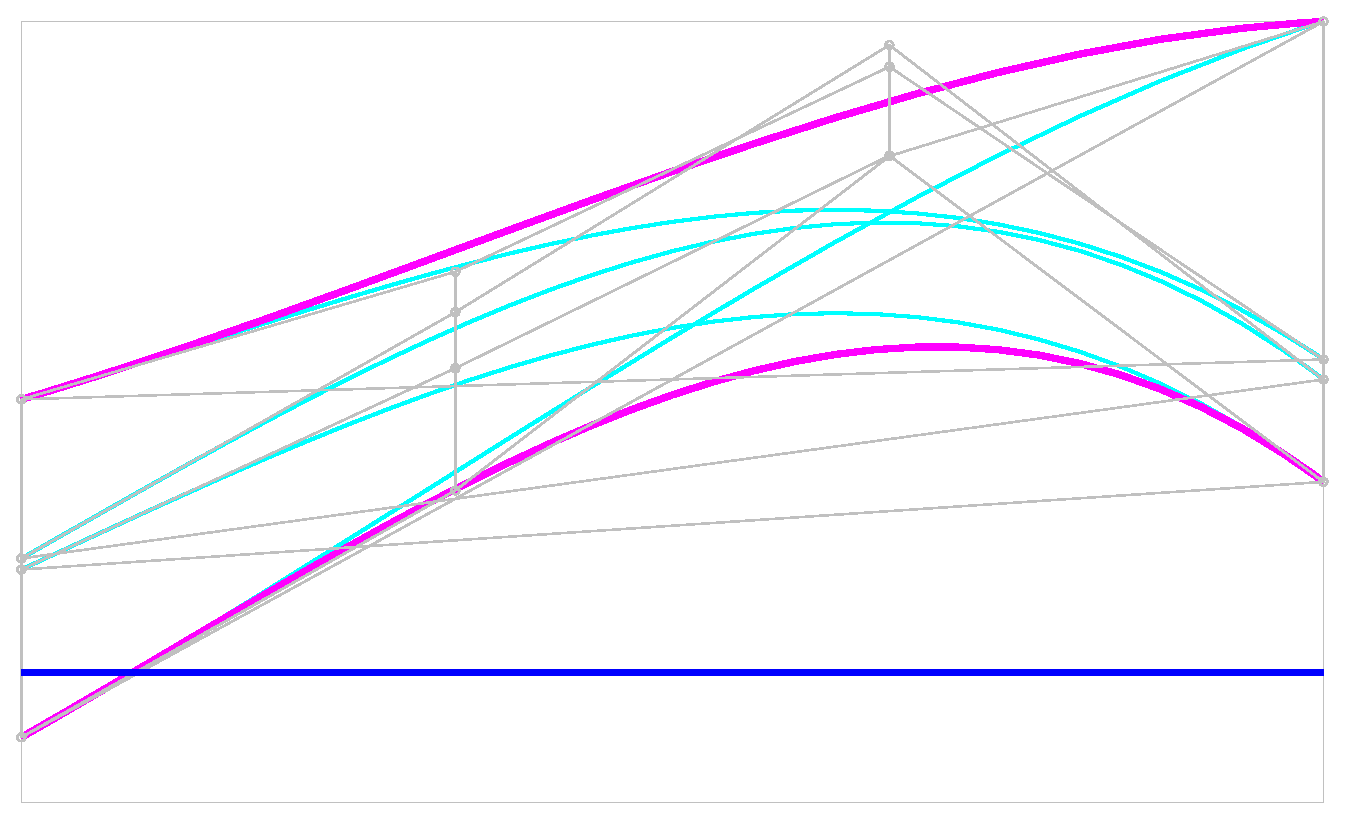
\includegraphics [ width=0.4\textwidth ]{pic/converted-bclip2_minmax.eps}
	\caption{The explicit patch along with its minimum and maximum curves. Notice that the projected distances on the left side of the patch diverge in sign, causing this side to be reset to zero during the ROI search}
	\label{fig:minmax}
\end{figure}

\subsection{Lighter ROI search - min/max curves only instead of complete convex hull test}
\label{sec:bc_minmax}
Since Bézier surface is basically an interpolation between four control curves, it is obvious that any object bounding projections of all the control curves also bounds the projection of the entire surface. Taking this logic a bit further, we can see that if we collect minimum and maximum among corresponding control points of all four control curves, resulting min/max curves will bound the whole explicit patch (figure \ref{fig:minmax}). In fact, this is equivalent to treating the explicit patch as an interval Bézier curve (\cite{Sederberg92approximationby}).

Thus, instead of testing the full projected convex hull, we can compute the ROIs from just two curves - minimum and maximum, and then merge them. To our experience, the resulting ROI quality degrades just slightly, but the ROI search procedure becomes significantly faster.

\subsection{Half clipping - one side clipping only if other side is reset}
Experiments revealed that quite frequently the projected distance signs diverge at one side of the convex hull (like left half on the figure \ref{fig:minmax}). In such a case, the corresponding ROI end must be reset to zero or one, appropriately. Accordingly, patch clipping from the reset side becomes excessive and can be skipped, saving the half of clipping operations. During the ROI search, we keep track of this fact and set either left or right side flag, or both - depending on the situation. The last case leads to performing a patch split instead of the search and clipping, and for the other two cases we use a reset-aware clipping procedure, where those flags are passed to. In our experiments, such a reset-aware clipping was able to save up to 5\% of total rendering time, depending on the scene.

\subsection{Early miss based on the distance span bounds signs}
Similar to \cite{Tejima2015subdivision}, as a byproduct of computing parametric line distances, we keep track of distance signs. If all the distances have the same sign, the patch doesn’t overlap direction line at all, so miss is immediately reported.

\subsection{Performance comparison}
We've implemented both the original Bézier Clipping and the optimizations enlisted here in a C++ program using a single precision scalar floating point math.

Our test application is quite simplified and designed solely to serve as a testbed for ray/patch intersection algorithms. We trace primary rays only and don't construct any acceleration structures at all, to avoid their influence on rendering time. Instead, we perform a simple screen-space binning/depth sorting of the patches and use z-buffering inside the bin to find the nearest intersection point during the rendering. Thus, rendering performance is entirely determined by the performance of ray/patch intersection procedure.

Our test scenes database has been converted and compiled from publicly available models (partially from sPatch/HamaPatch files, partially from Catmull-Clark subdivision surfaces in various modeling software formats).

We compiled the program on Windows 10 platform using MS Visual C++ 2022 and run both original and modified rendering versions on AMD Ryzen 9 3900X CPU @3.8 GHz. The resulting timings provided in the table \ref{tbl:bc_test_num} clearly demonstrate the performance effect from the optimizations above.


\section{GeoClip specific modifications}
North's GeoClip is a substantial algorithmic improvement over the original Bézier clipping. Essentially, it employs so called hybrid Bézier curves as the quadratic bounds of the projected distance patch. Then, the roots from solving two quadratic equations are taken pairwise to provide one or two ROIs. Such an approach is well suited for the cases where original Bézier Clipping fails to react optimally and produces excessive patch splitting, causing severe performance penalty - intersections near the silhouette edges, sharp patch corners and singularities. GeoClip naturally avoids such a splitting, either reporting a miss or producing nice and tight double intervals for highly curved patches right away. GeoClip also tends to produce much tighter ROIs than Bézier Clipping even for single interval case, due to the fact that quadratic bounds are able to better follow the shape of the curved patch projection.

Of course, the first thing that should be mentioned or emphasized once more when discussing GeoClip (as well as other similar algorithms that employ quadratic bounds) is that the simplest and fastest naive implementation of quadratic solver isn't applicable here. Numerically stable solver is absolutely necessary. Failure to use it immediately results in false misses and other artifacts. One simple yet efficient solving technique is described in \cite{HornQuadratic}. Upon closer examination, it boils down to just a few additional operations on top of naive implementation and can be rearranged to avoid branches. This feature is important for SIMD implementation.

Another fact worth noting is that GeoClip ROI search complexity goes beyond just quadratic bounds generation and solving. The search procedure also contains such  unavoidable stages as root validation and sorting, needed to make sure that only those roots are taken that fall into a valid parametric range, and all valid roots are properly rearranged to correctly represent the ROIs. Those stages also bring a substantial computation cost, which is comparable to the cost of the quadratic solver itself. This severely increases the GeoClip iteration cost over the Bézier Clipping. So, to keep the algorithm competitive, this cost increase has to be paid off by producing much tighter ROIs, which should result in a substantially decreased number of the following iterations. But, intuitively, the discussion above suggests that certain conditions regarding the scene content must be met for allowing the GeoClip to show its best qualities.
Unfortunately, Utah teapot was the only thoroughly investigated use case in the original thesis. Further experiments revealed a quite unexpected GeoClip behavior feature discussed in subsection \ref{sec:flexclip}.

Since low level details of the author's GeoClip implementation were not included in the original thesis, it is hard to decide whether a given algorithmic optimization was already implemented by him or not. So we are adding all the details that weren't explicitly mentioned in the original work, but, to our opinion, play an important role in algorithm performance or robustness and stability.

\subsection{Bounds generation from precollected min/max intervals}
Original GeoClip computes the bounding curves by calculating and collecting midpoint intervals from all four control curves that define the patch.
Following the similar optimization for Bézier Clipping from section ~\ref{sec:bc_minmax}, we precollect the intervals for the explicit patch - i.e. compute min/max bounding curves first, and only after that we generate the bounds from those two curves.
This saves a substantial amount of computations compared to the original method, while difference in bounding curves produced is barely noticeable.

\subsection{Tighter bounding curves}
In his thesis\cite{NORTH07}, North proposes to represent a cubic curve or projected patch as an interpolation between a pair of quadratic bounding curves. Having a cubic Bézier curve $C$ with control points $P_{0}$,$P_{1}$,$P_{2}$,$P_{3}$, to obtain those quadratic bounding curves $C_{1}$ and $C_{2}$, he takes the endpoints as is and generates midpoints using the following equations:

\begin{align*}
%\[
P_{mid,1}=\frac{1}{2}P_0+\frac{3}{2}P_1
%\]
&&
%\[
P_{mid,2}=\frac{1}{2}P_3+\frac{3}{2}P_2
%\]
\end{align*}

The formulas are extremely simple and very fast compared to most of the other proposed approximation methods. But, due to their nature, bounds generated this way can't always closely follow the initial curve shape direction. Each of them is only able to tightly enclose one of the curve ends. So, a fairly large distance remains between them and the rest of the bounded curve. This disadvantage especially vividly manifests itself if the bounded curve has an inflection point, cusp, or other singularities.

\cite{Yzerman20simplify} proposed an alternative named \emph{midpoint approximation} (North's bounds turn out to be an equivalent to Yzerman's \emph{endpoint approximations}). Following the proposal, we generate a single approximating curve $C_3$ by averaging the two midpoints above and obtaining the central point $P_{mid,3}$:
\[
P_{mid,3} = \left(1 - \frac{1}{2}\right)P_{mid,1}+\frac{1}{2}P_{mid,2} = \frac{1}{4}\left(3P_1-P_0+3P_2-P_3\right)
% = \frac{1}{4}\left(3\left(P_1+P_2\right)-\left(P_0+P_3\right)\right)
\]
Then, we compute a maximum parametric distance from the approximating curve to original cubic one:
\[
d_{max,3}=\frac{1}{12\sqrt{3}}\left(P_0-3P_1+3P_2-P_3\right)
\]
and then, after shifting $C_{3}$ up and down by this distance, a pair of new bounding curves can be obtained:
\[
{\hat{C}}_{31,32}=C_3 \pm d_{max,3}
\]
The bounding curves for the whole projected surface patch are computed in a manner similar to the original method. Instead of the degenerate interval above (single cubic curve), bounds generator accepts the interval representation of the whole patch, and outputs the upper shifted bound from the maximum curve and, accordingly, the lower bound from the minimum.

Since the new midpoint $P_{mid,3}$ lies much closer to the original curve and new approximation error bound $d_{max,3}$ is more than three times smaller than for North's $C_{1}$ and $C_{2}$, new bounds much better follow the initial patch shape and enclose it much tighter, with almost the same, minimal computational complexity of generation. Thus, such bounds produce tighter ROIs and faster report misses, saving a substantial number of subsequent iterations.
Some examples coming from our testing experience demonstrate the advantages of this new approach (figure \ref{fig:tighter_bounds}).
\begin{figure}
	\centering
	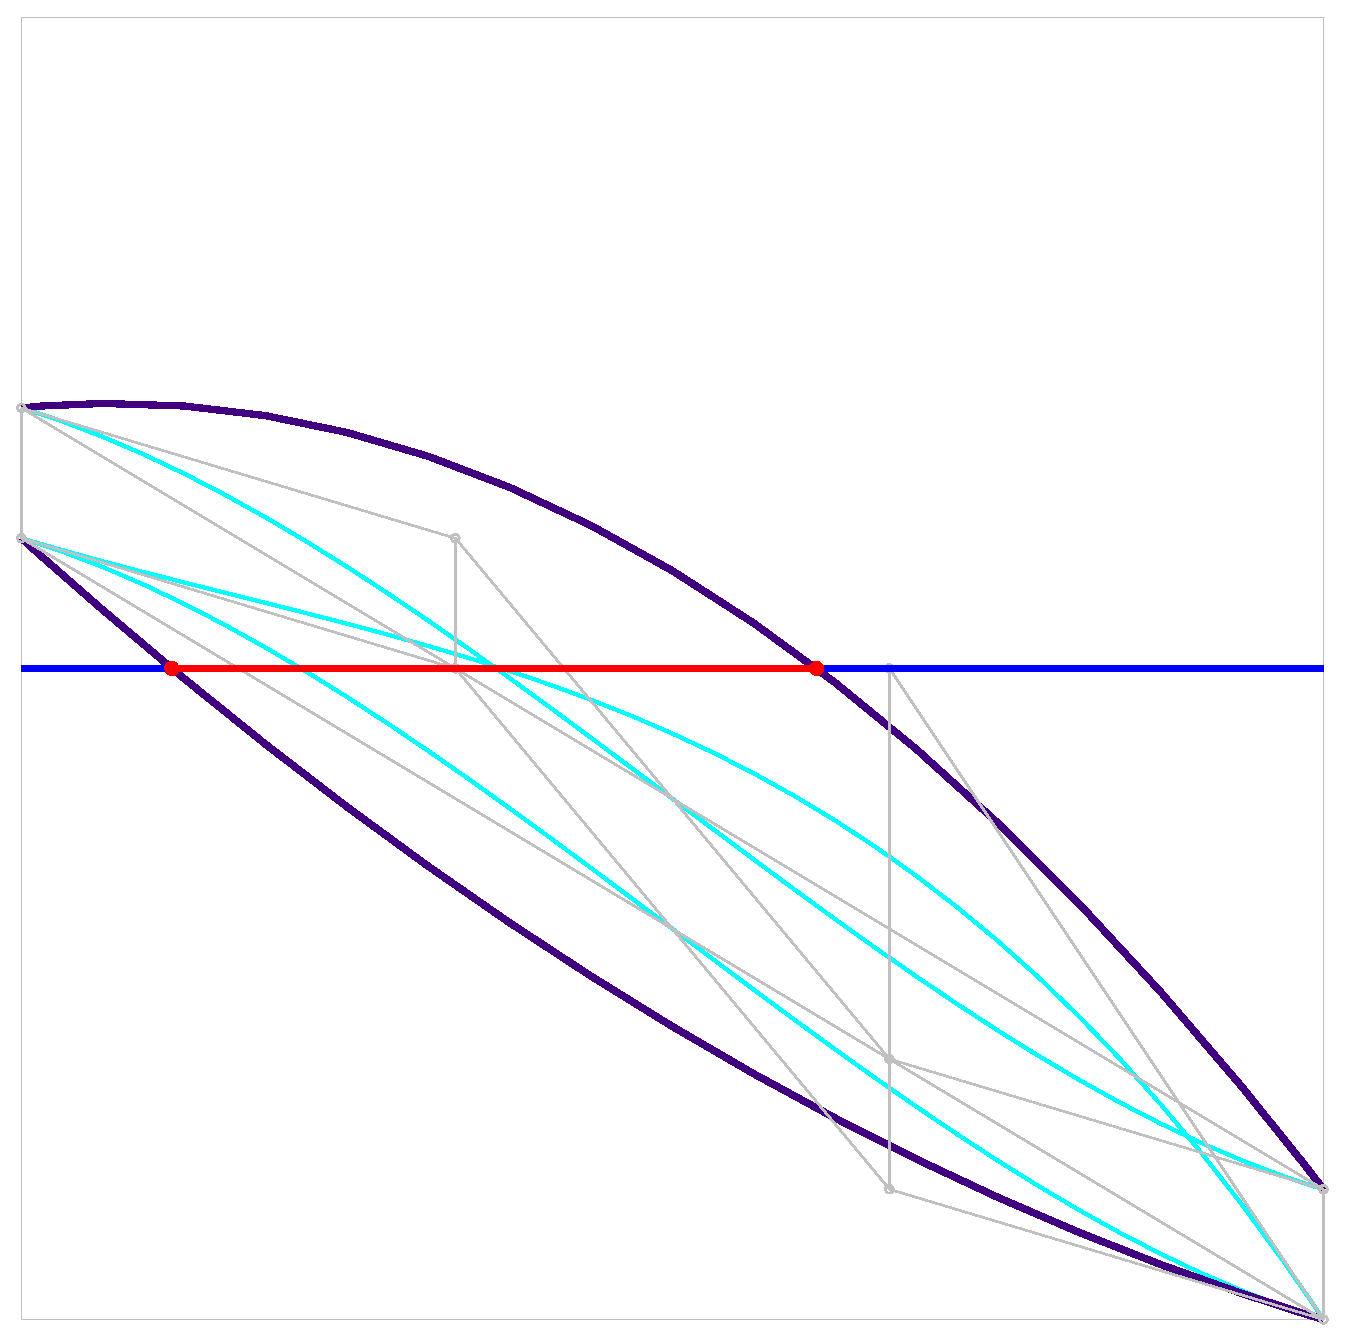
\includegraphics [ width=0.24\textwidth ]{pic/tighter_bounds_showcase/1/converted-classicU.eps}
	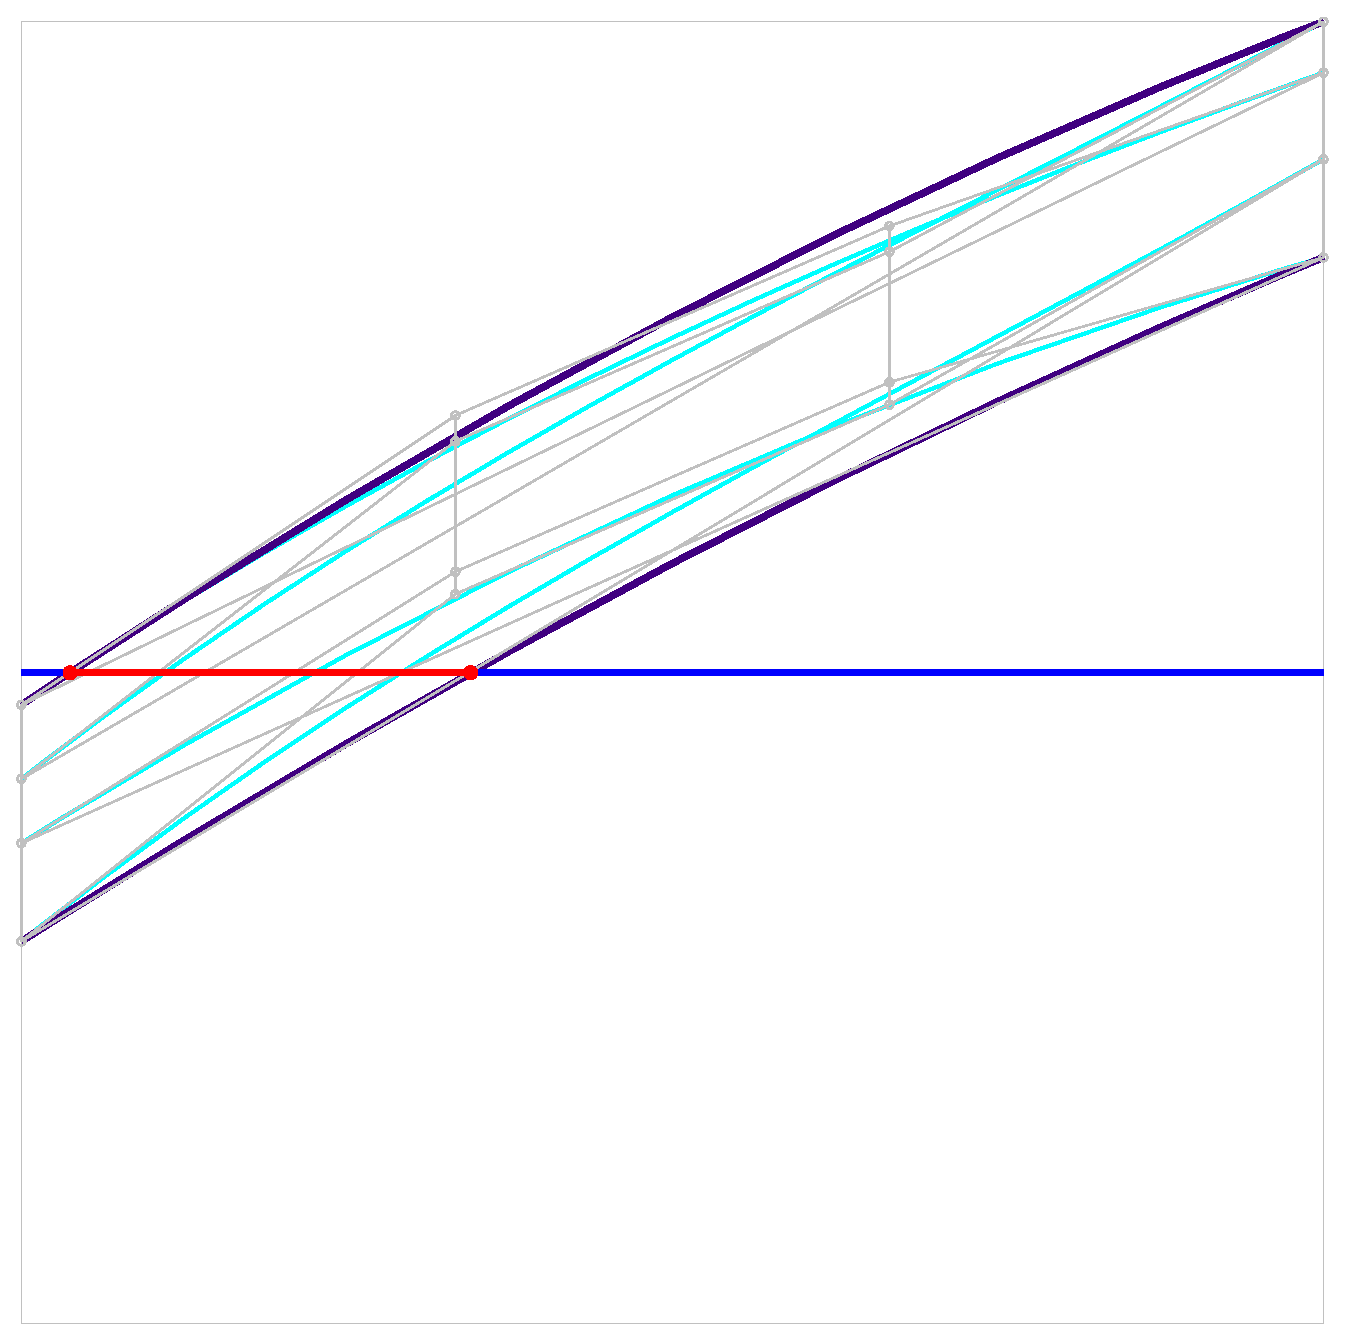
\includegraphics [ width=0.24\textwidth ]{pic/tighter_bounds_showcase/1/converted-classicV.eps}
	\hfill
	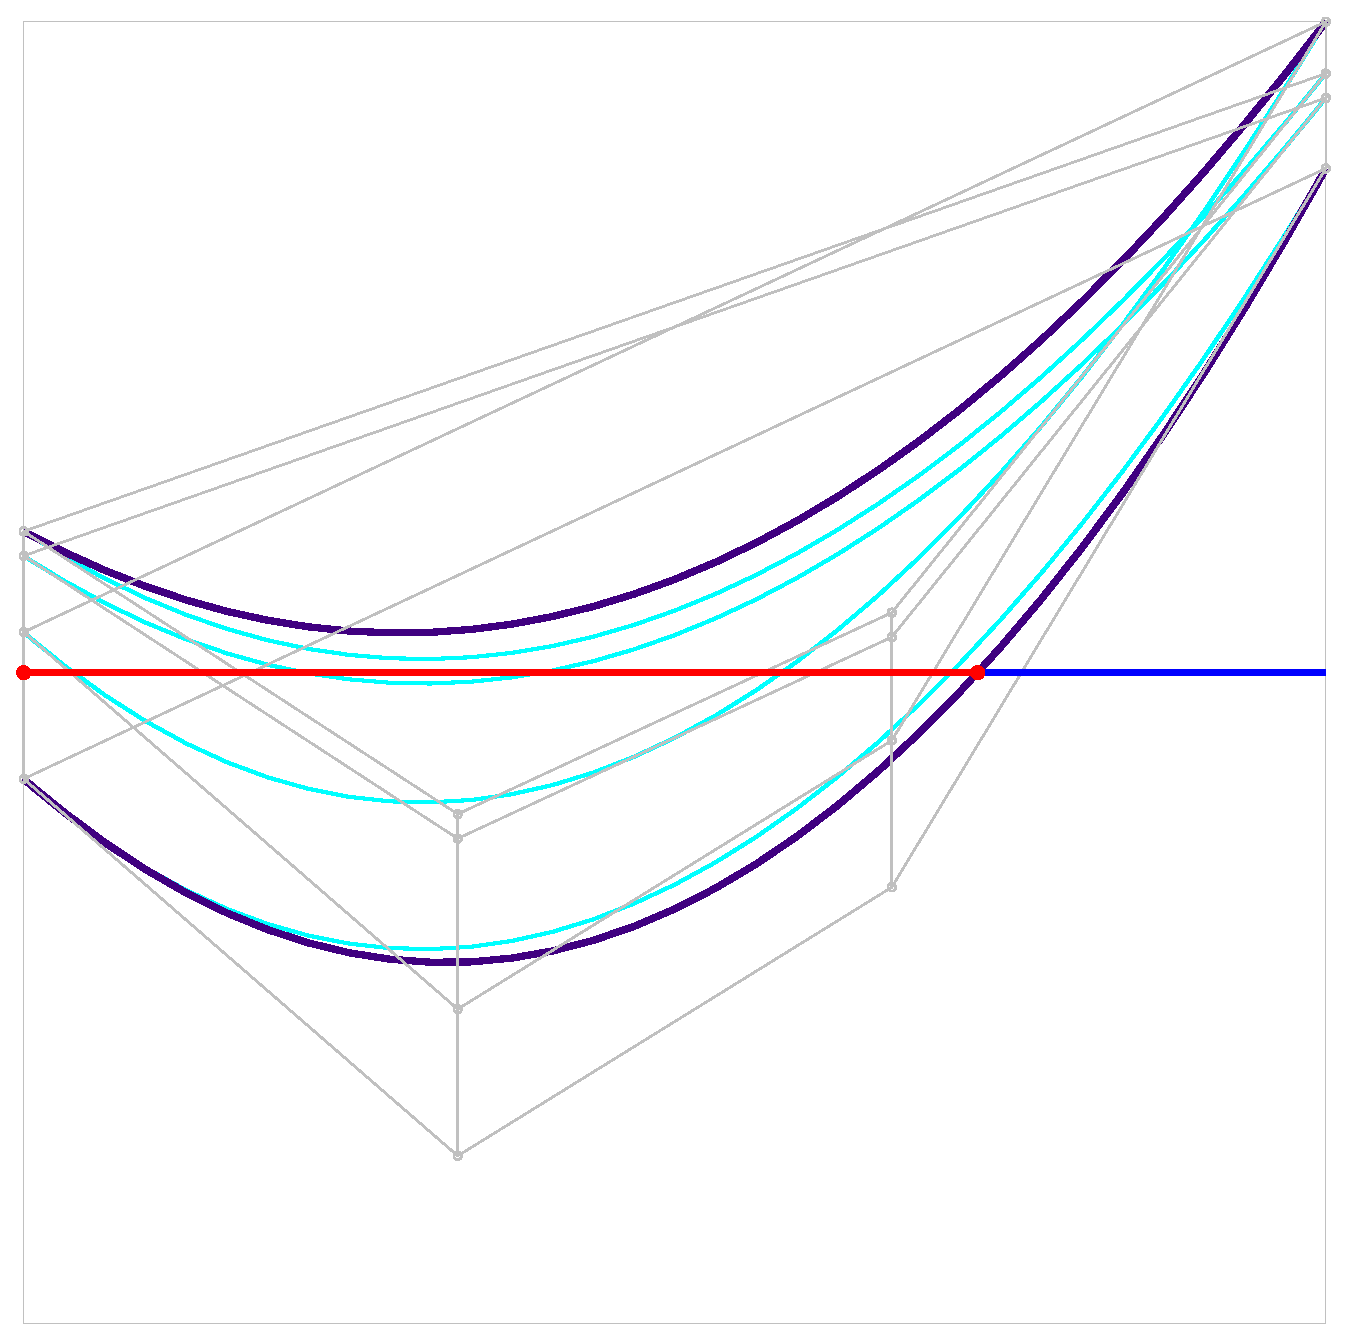
\includegraphics [ width=0.24\textwidth ]{pic/tighter_bounds_showcase/4/converted-classicU.eps}
	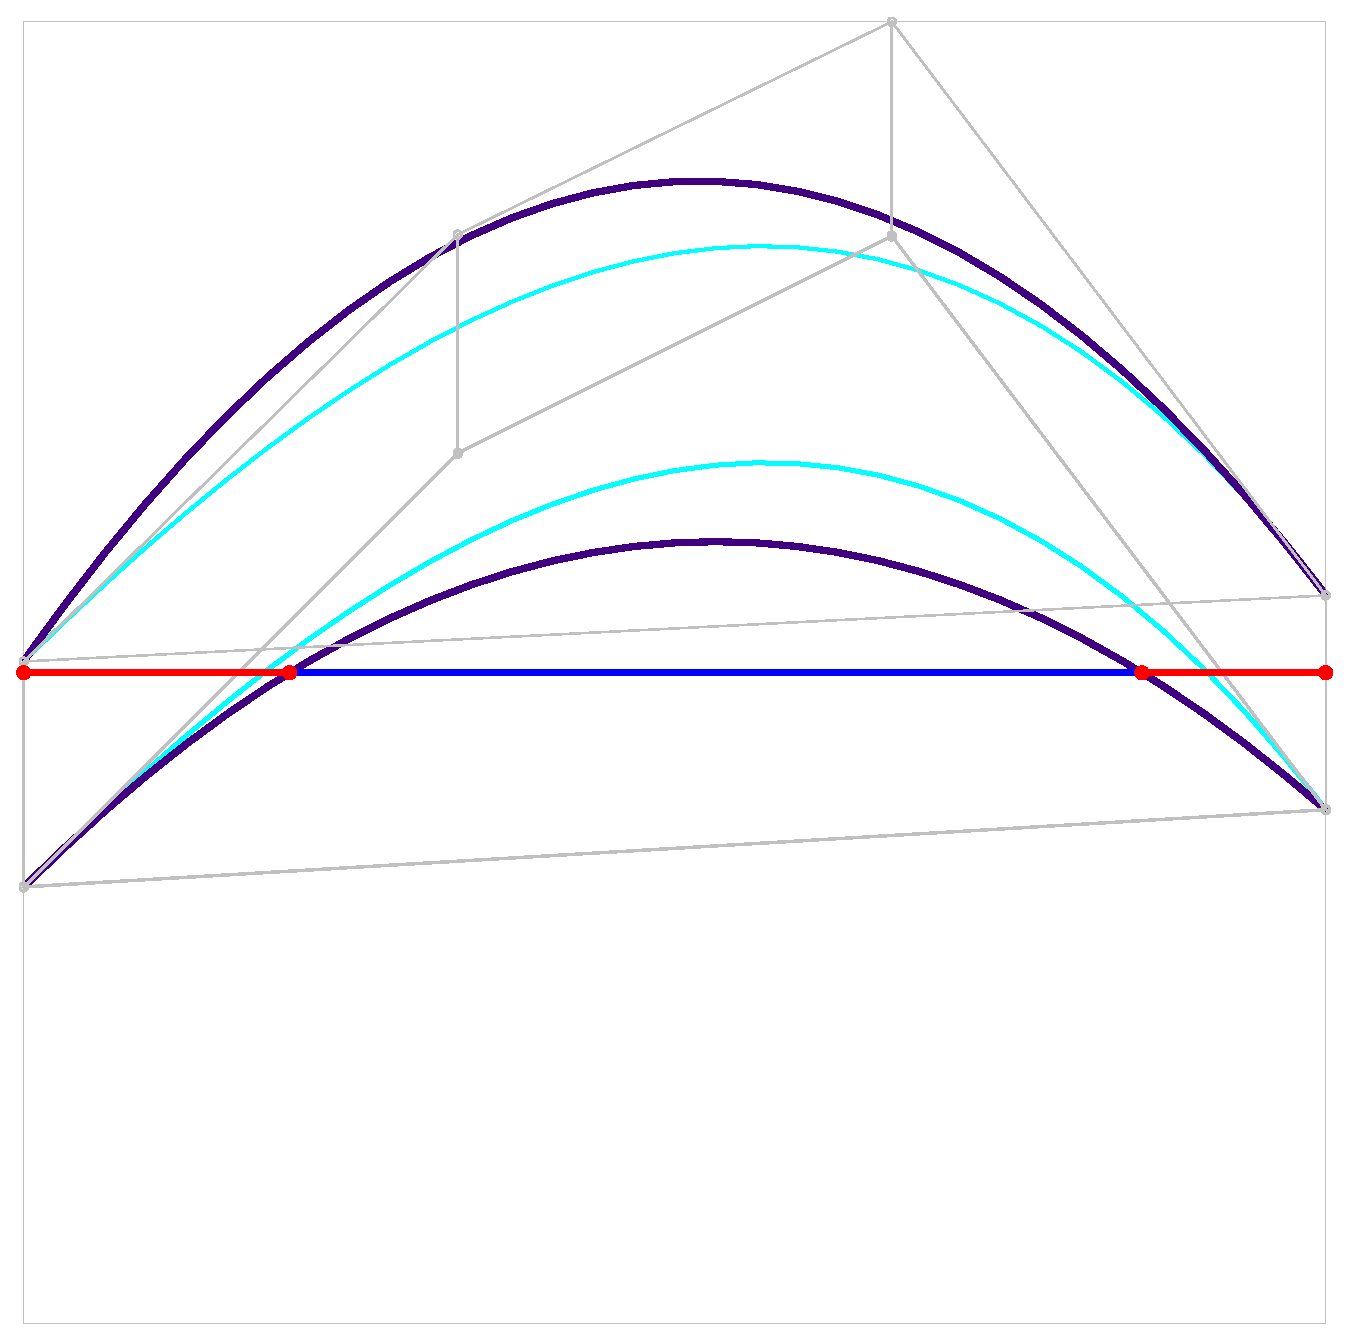
\includegraphics [ width=0.24\textwidth ]{pic/tighter_bounds_showcase/4/converted-classicV.eps}
	\\
	\includegraphics [ width=0.24\textwidth ]{pic/tighter_bounds_showcase/1/converted-newU.eps}
	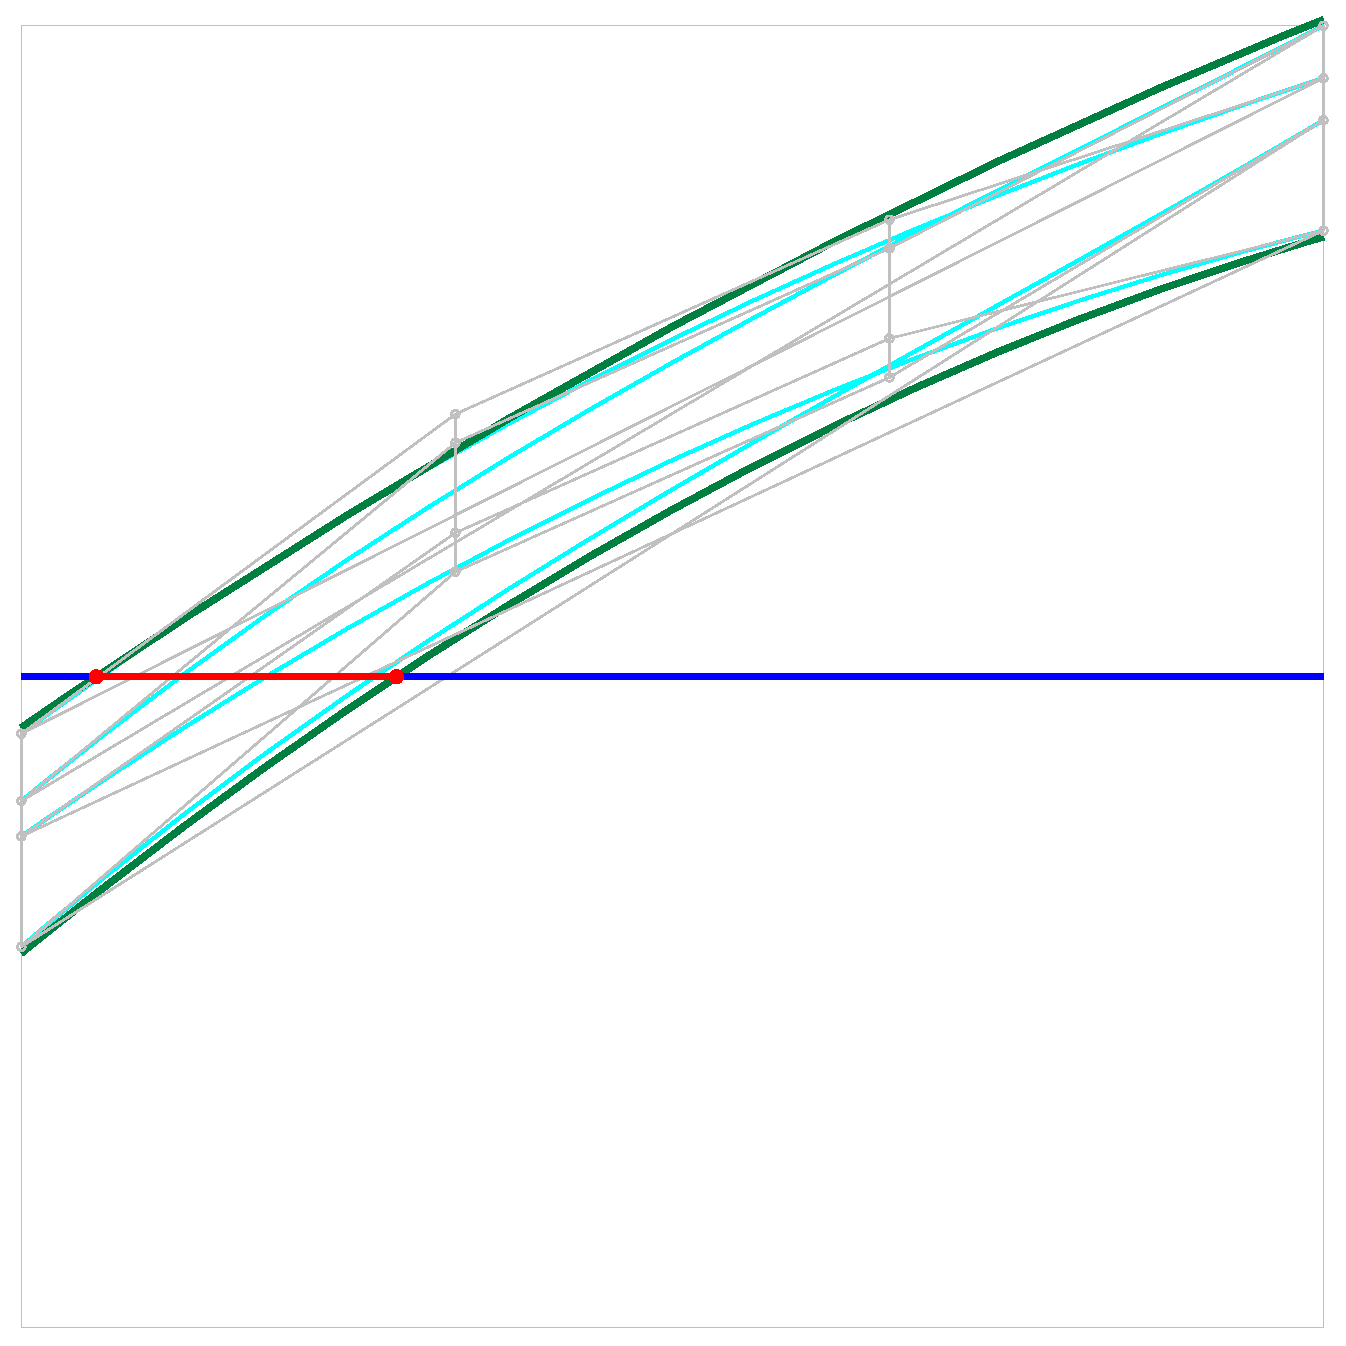
\includegraphics [ width=0.24\textwidth ]{pic/tighter_bounds_showcase/1/converted-newV.eps}
	\hfill
	\includegraphics [ width=0.24\textwidth ]{pic/tighter_bounds_showcase/4/converted-newU.eps}
	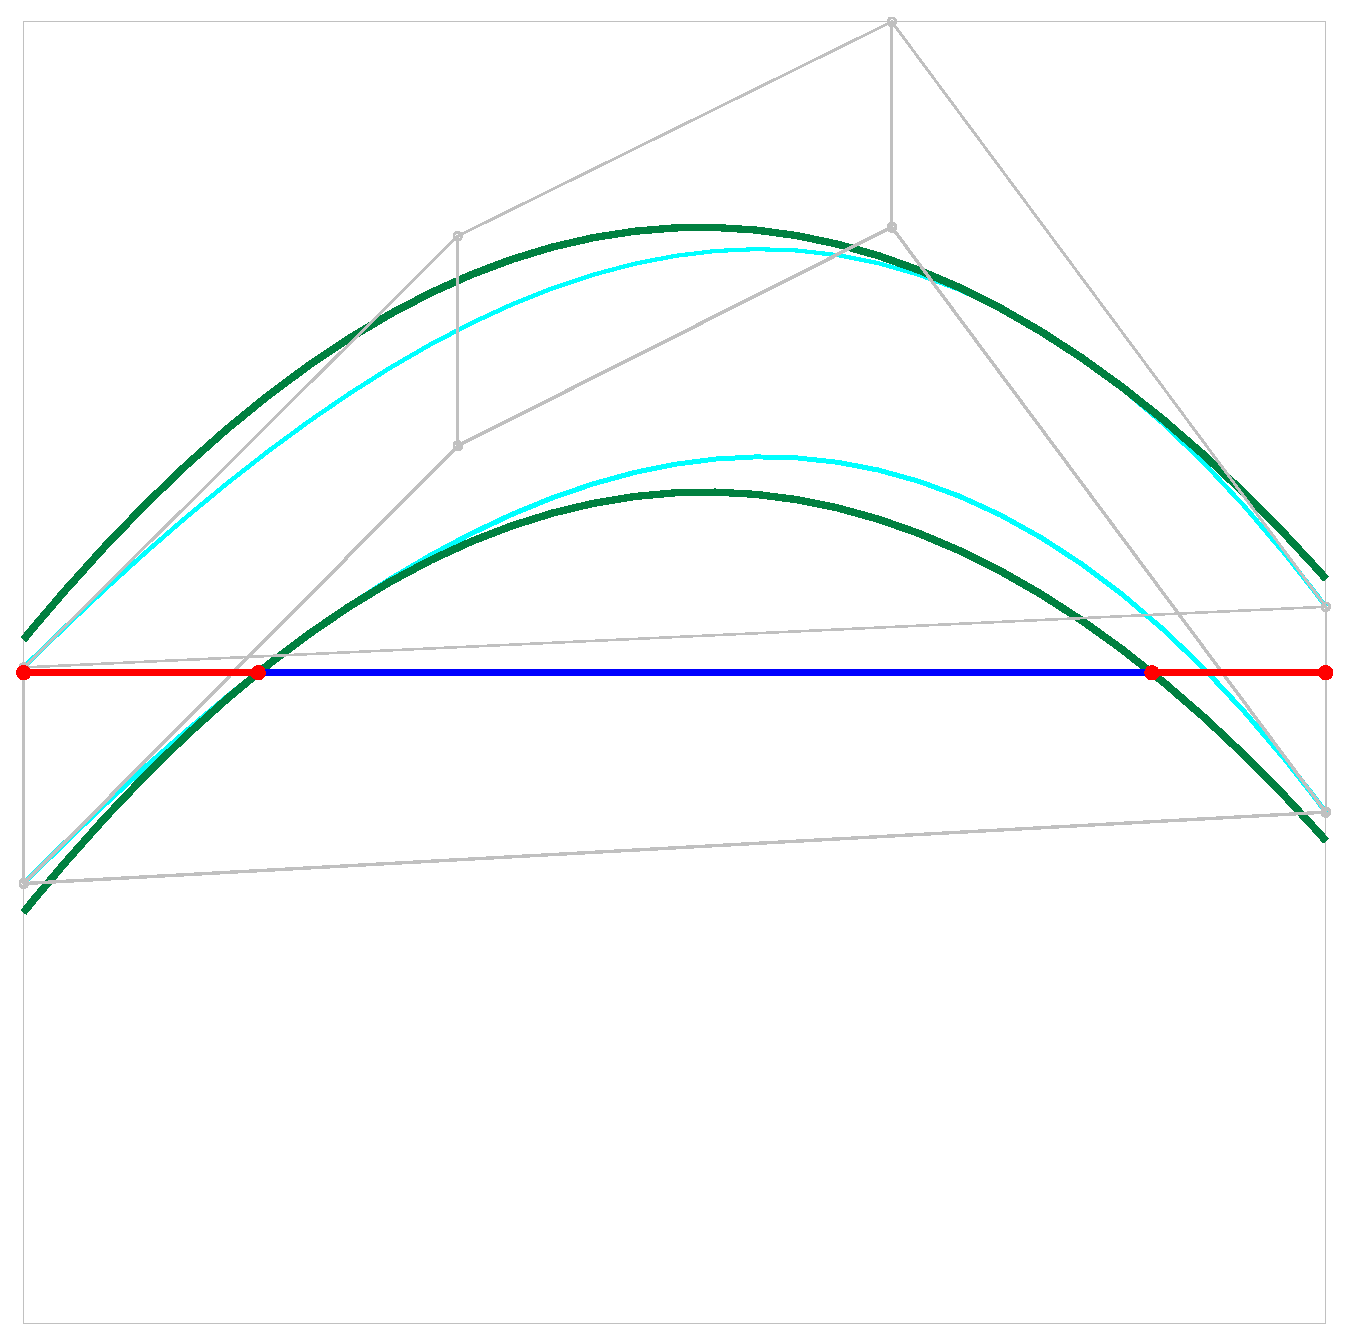
\includegraphics [ width=0.24\textwidth ]{pic/tighter_bounds_showcase/4/converted-newV.eps}
	\\
	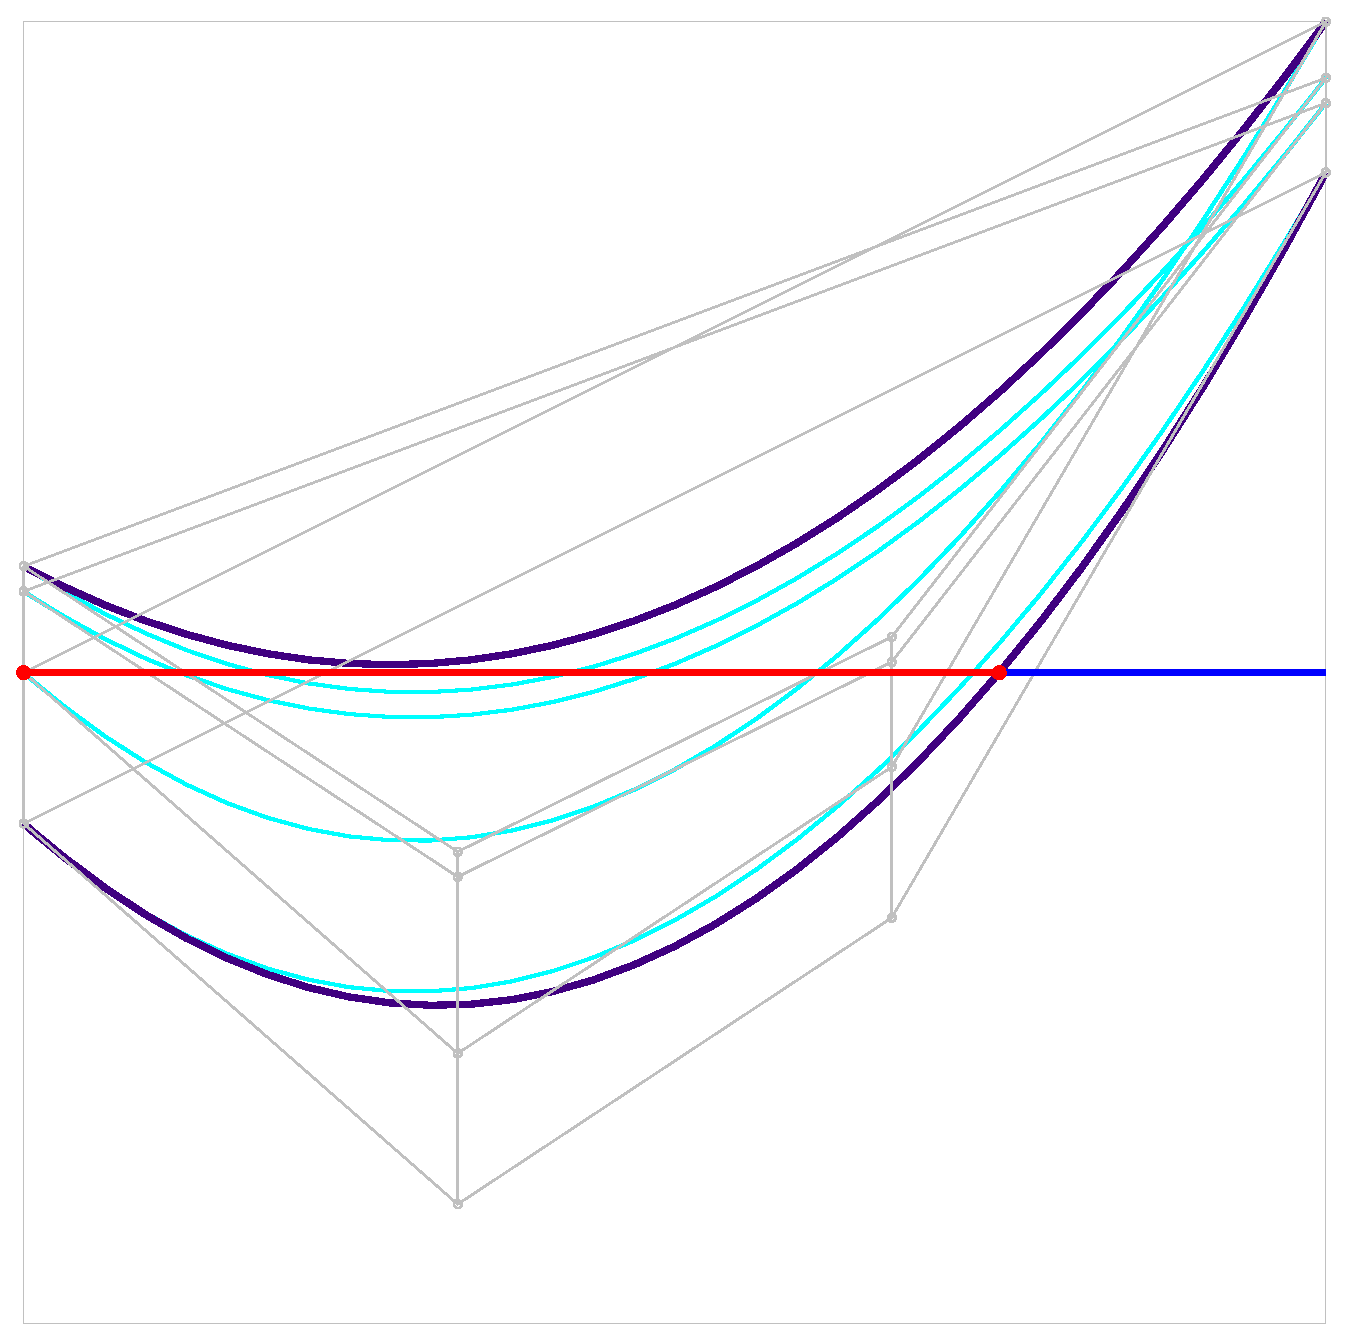
\includegraphics [ width=0.32\textwidth ]{pic/tighter_bounds_showcase/2/converted-classicU.eps}
	\hfill	
	\includegraphics [ width=0.32\textwidth ]{pic/tighter_bounds_showcase/3/classicV.eps}
	\hfill
	\includegraphics [ width=0.32\textwidth ]{pic/tighter_bounds_showcase/5/classicV.eps}
	\\
	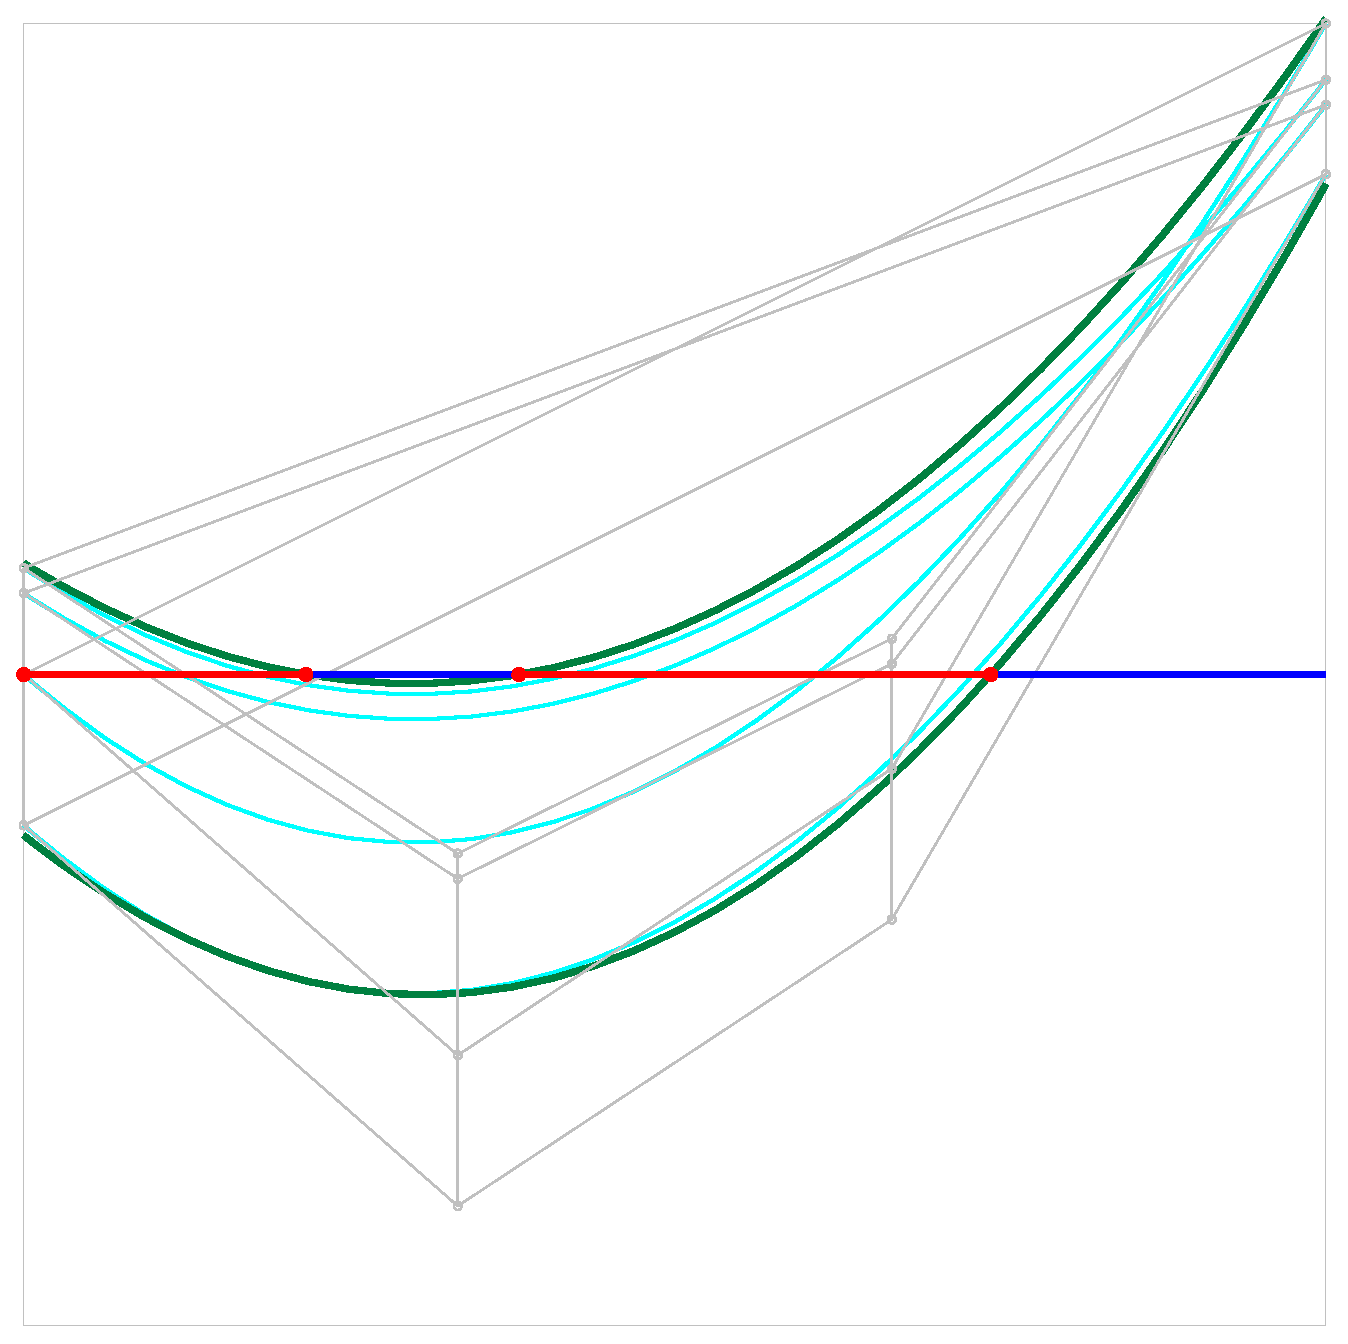
\includegraphics [ width=0.32\textwidth ]{pic/tighter_bounds_showcase/2/converted-newU.eps}
	\hfill
	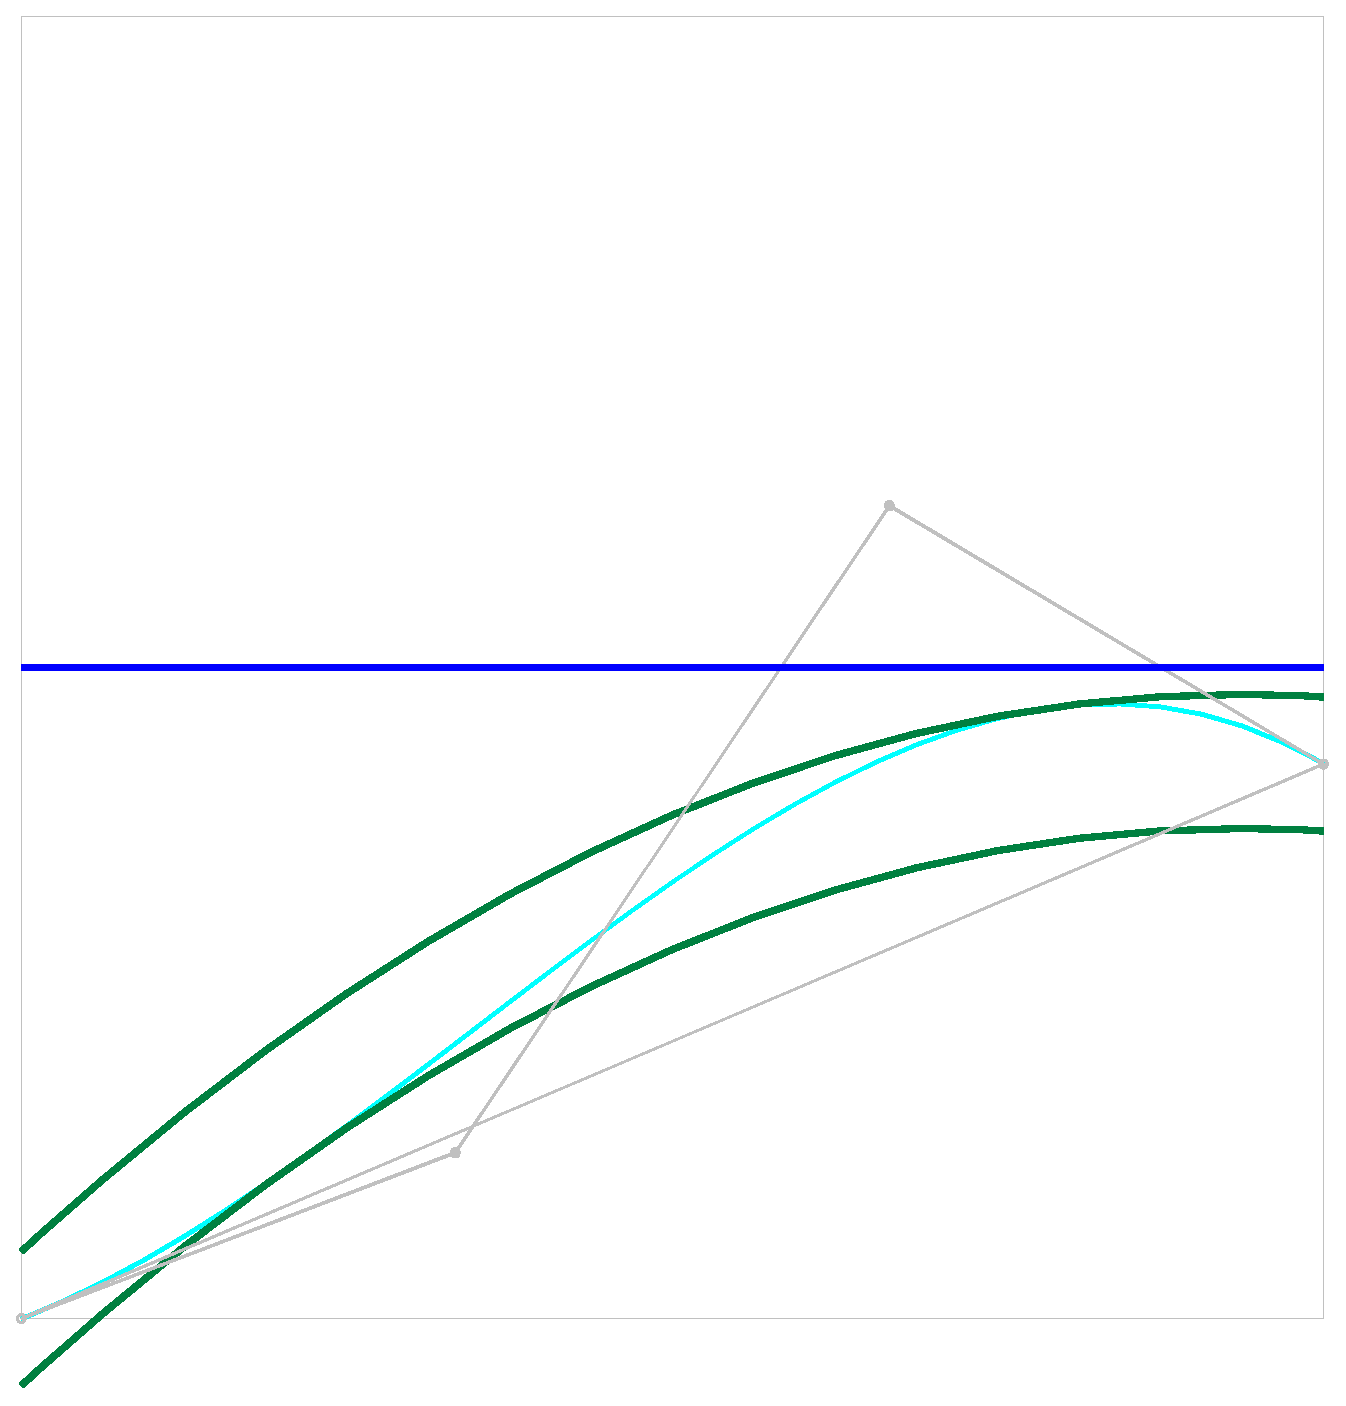
\includegraphics [ width=0.32\textwidth ]{pic/tighter_bounds_showcase/3/newV.eps}
	\hfill
	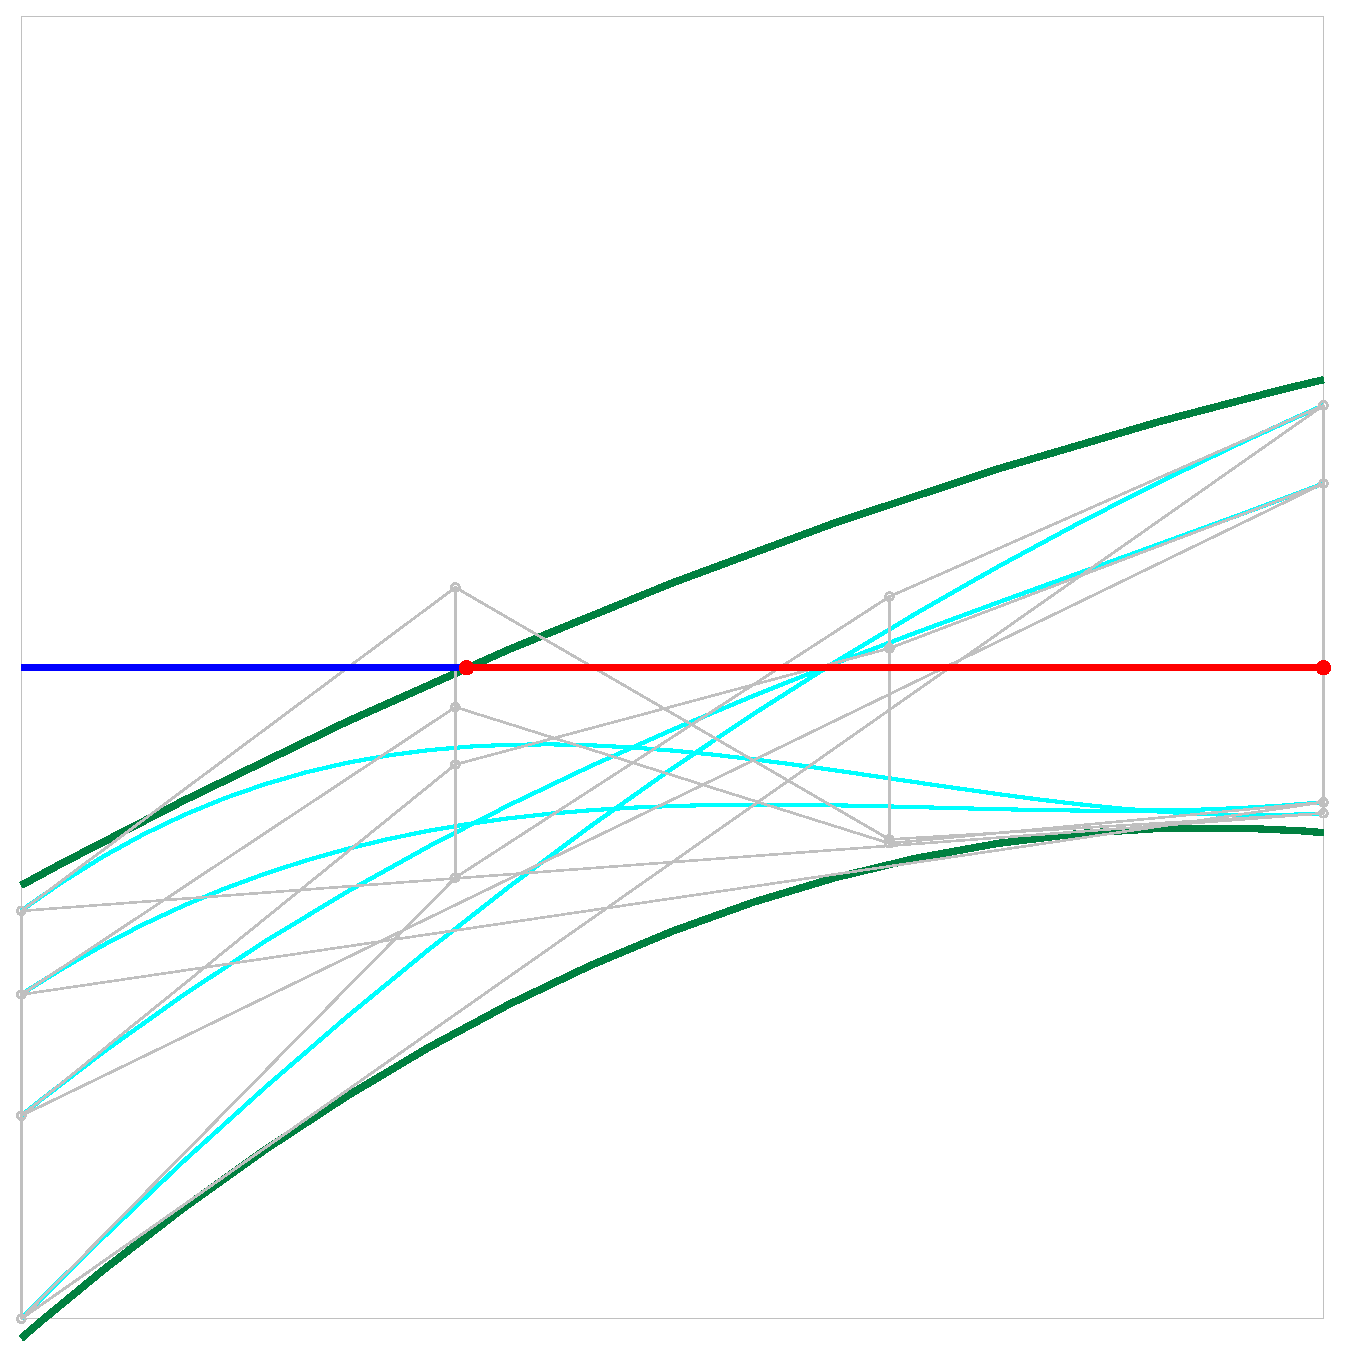
\includegraphics [ width=0.32\textwidth ]{pic/tighter_bounds_showcase/5/newV.eps}
	\caption{Several examples of ROI search from rendering our test models with original and newly proposed bounding curves. The original bounding curves are shown with violet in upper row, the new bounds for the same projected patch are shown with dark green in a lower row. Notice how new bounding curves produce tighter ROIs which result in a better convergence on current or following iteration, split a single long ROI into two tighter parts, and create a miss instead of scraping the small ROI, preventing from continuing further iterations. }
	\label{fig:tighter_bounds}
\end{figure}

\subsection{Preliminary convex hull/zero line overlap test for bounds}
Since generated quadratic bounds are also Bézier curves, convex hull property still holds for them too. So, before starting an expensive work like converting the curve coefficients and calling the quadratic solver, a simple and quick test for zero overlap can be performed. If the sign of the central point distance is different from any of two ending points, then the curve might have roots, and we proceed further. If all three signs are the same, this parabola has no roots for sure, and we skip it. The test is just a couple of boolean operations, so it is extremely cheap, but proved very useful, often saving a lot of computations.

\subsection{Modified splitting threshold}
During our experiments we noticed that it is more beneficial to use 0.75 as a patch splitting threshold instead of a value 0.8 recommended by all original authors. To our experiments, such a modification tends to eliminate some extra iterations and brings a small, but stable performance benefit, which is about 0.5-1\%.

\subsection{Deferred and rearranged patch processing}
In contrast to Bézier Clipping, the patch processing logic of GeoClip, which follows the ROI search, is more sophisticated than just deciding whether we should clip or split in current dimension. We might receive one or two ROIs in both U and V dimensions, plus, in case of a single ROI, we still need to account for possible splitting. To correctly process this, we may need to perform a uni- or bidirectional split and/or uni- or bidirectional extraction of subpatches.
Each patch processing procedure is rather expensive by itself, but their relative costs are different. For example, compared to splitting, clipping has double cost, and subpatch extraction has almost quadruple. So, to minimize the total processing cost, it is important for the logic to do things in a right order - to prefer duplicating cheaper operations instead of costly ones.

Here we apply the following rule: if only the clipping is required - it is performed immediately after the search, otherwise - the processing is delayed until the exact situation becomes defined in both dimensions. Then, once we're done with ROIs for both parameters, the pending subpatch extractions are performed if necessary, then splits.

\begin{figure}[t]
	\centering
	\includegraphics [ width=0.3\textwidth ]{pic/kirche_closeGeo_close.png}
	\hfill
	\includegraphics [ width=0.3\textwidth ]{pic/pyramidGeo_close.png}
	\hfill
	\includegraphics [ width=0.3\textwidth ]{pic/sauele_allGeo_close.png}
	\caption{Problematic scenes for the GeoClip algorithm}
	\label{fig:geohard}
\end{figure}

\subsection{Adding more flexibility - switching to linear ROI search}
\label{sec:flexclip}
When the form of one of the bounding parabolas happens to be close to linear, the denominator for one of the roots approaches zero. This creates a risk of overflow that we definitely want to avoid. So, when denominator drops below a certain threshold, we have to stop using a quadratic solver and switch to some other safe solution.

Also, during the GeoClip comparative performance testing against Bézier Clipping, it became obvious that scenes featuring large flat (or close to flat) patches are problematic for the GeoClip algorithm (figure \ref{fig:geohard}). This happens because the explicit patch projections of such flat patches are very close to linear. Thus, Bézier Clipping piecewise-linear convex hull search algorithm provides tighter ROI in less time, while GeoClip's attempts to tightly enclose a linear domain with parabolas turn out to be just a waste of time. Not surprisingly, GeoClip not just fails to provide a stable speedup on such scenes, but sometimes even struggles to achieve the same performance as Bézier Clipping. Interesting side note here is that actually a large percentage of the scenes converted from Catmull-Clark subdivision models, that we had a chance to test, tend to contain mostly patches that are close to flat, so GeoClip exhibits a similar behavior on them.

It is also a well known fact that, despite of the initial patch form, as clipping iterations proceed, the resulting patch becomes more and more flat, producing more and more linear-like projected convex hull and making the GeoClip approach less and less effective. When the ratio of such iterations grows over some limit, the GeoClip starts demonstrating a slowdown, like on the examples above.

\begin{figure}[t]
\centering
	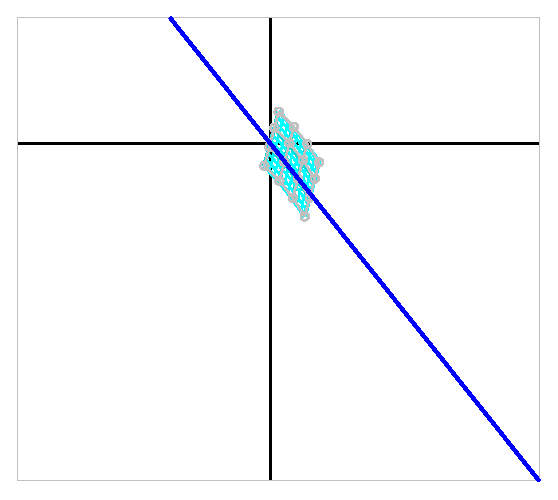
\includegraphics [ width=0.3\textwidth ]{pic/linear/geoclip5.eps}
	\hfill
	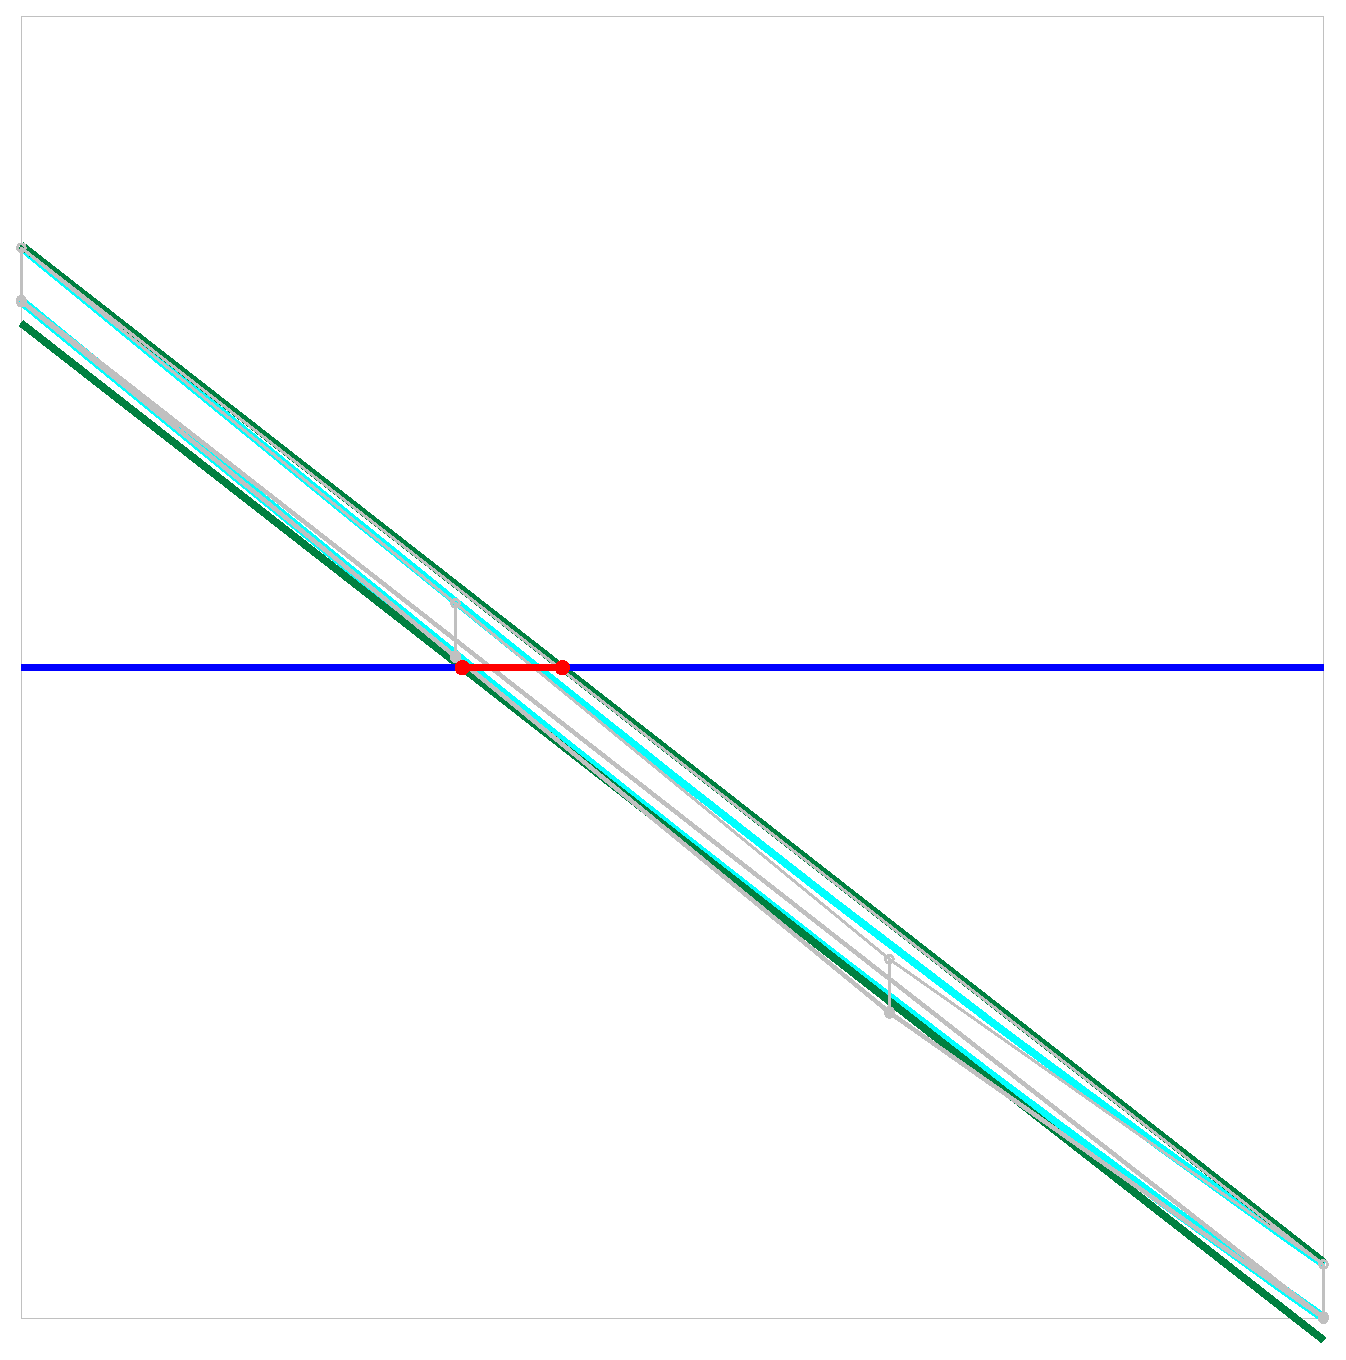
\includegraphics [ width=0.3\textwidth ]{pic/linear/geoclip6.eps}
	\hfill
	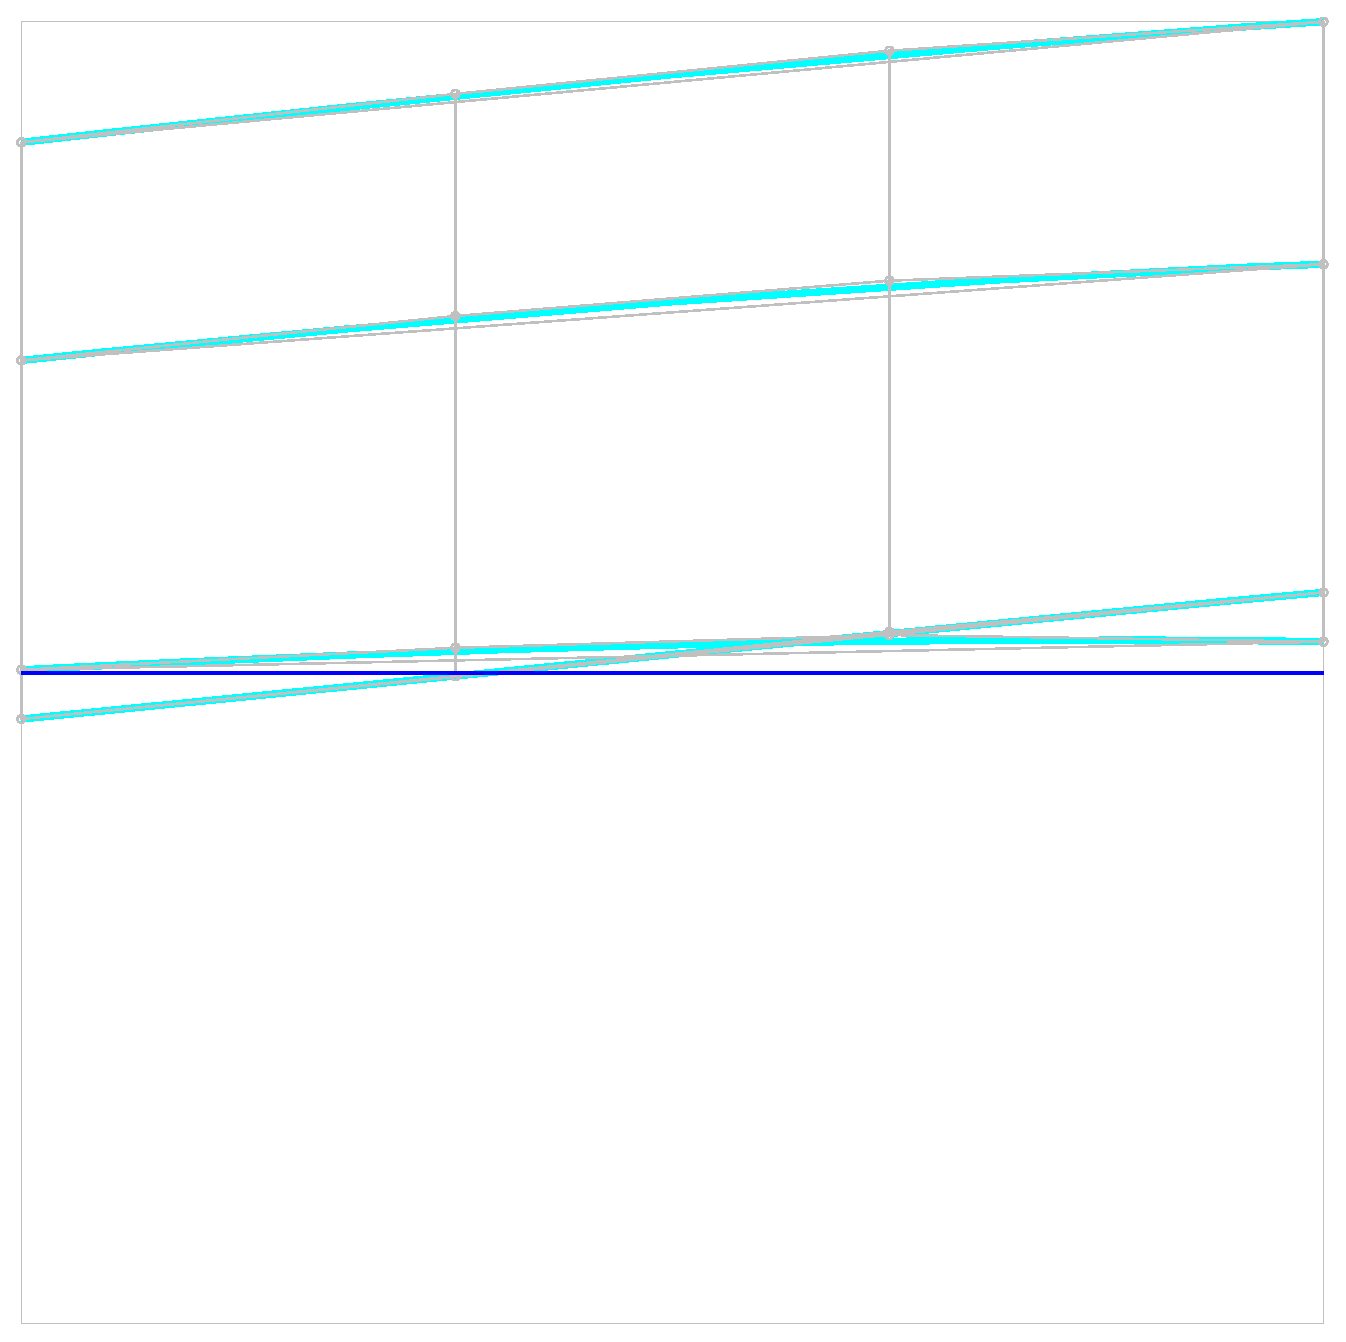
\includegraphics [ width=0.3\textwidth ]{pic/linear/geoclip7.eps}
   \caption{\label{fig:linear_search}
     Cases which lead to to the linear search switch - flat patch example, new linear bounds for it along with ROI detected, and "thick" explicit patch example }
\end{figure}

In order to close the algorithmic gaps described above, we decided to add a new procedure of linear parameter ROI search. Instead of the original piecewise convex hull or quadratic parabolas, this algorithm uses two straight lines, which are the outer borders of fat lines produced by minimum and maximum curves.
For each curve we choose one of the two parametric distance extrema - that one which shifts farther to the outside from the curve central line $P_0P_3$. In case if the curve is concave and both distances shift inside, the central line itself is taken:
\begin{align*}
%\[
\centering
d_1 = 3P_1 - 2P_0 - P_3
%\]
&&
%\[
d_2 = 3P_2 - 2P_3 - P_0
, \\
d_{border,min} = min(d_{1, min}, d_{2, min}, 0)
%\]
&&
%\[
d_{border,max} = max(d_{1, max}, d_{2, max}, 0)
%\]
\end{align*}

Intersections of those border lines with zero level provide a single ROI (figure \ref{fig:linear_search}). Such a procedure is numerically safe, it is about 1.5-2x cheaper than Bézier Clipping search and about 4-6x cheaper than GeoClip. At the same time, when the convex hull shape is close to linear, this linear algorithm produces the same or sometimes even better quality ROI than Bézier Clipping.

We also switch to linear codepath in case of degraded curves and for the "thick" projected patches. The patch is considered "thick" when its curvature drops below the quarter of its "thickness". Such "thick" patches tend to produce just a one large ROI, which, most likely, will be split anyway because its length exceeds the splitting limit. So, calling a quadratic solver on such patches almost always is just a waste of time, and the linear search produces very similar ROI, but much faster.

As a criteria for switching from GeoClip quadratic parabolas to new linear bounds, we employ two simple heuristics taking into account three characteristics of the explicit patch - the absolute value of maximum parametric distances above $N_{max}=max(|d_{1,min}|,|d_{2,min}|,|d_{1,max}|,|d_{2,max}|)$ as a cheap measure of the patch curvature, the maximum of projected distances absolute values $d_{max}$, and, finally, the patch "thickness" $L_{max}$, which is a largest span between minimum and maximum among any four corresponding control points collected from the same position at all four control curves. The switch happens when either of the two following conditions holds:

\[N_{max}<0.2d_{max}\]
\[N_{max}<0.25L_{max}\]

The described switch heuristic is not strictly mathematically justified, but it is rather computationally inexpensive and works satisfactory on most scenes. When the projected patch convex hull becomes "linear" for U or V direction, we detect this fact and set an appropriate local boolean flag. Once the flag for a given parameter is set, we don't compute the heuristic anymore and continue permanent linear search for this parametric dimension until the intersection point is found.

Thus, the modified ROI search pseudocode becomes like the following:
\begin{itemize}
\item if the "flat" flag has been already set for this direction, go to linear search and return the ROI produced by it
\item based on $d_{ij}$, calculate $d_{max}$, $N_{max}$, $L_{max}$ and estimate the heuristic
\item if the heuristic returns true - set the flag and switch to linear search
\item else, proceed with GeoClip quadratic bounds solution
\end{itemize}

The linear search brings some overhead for heuristics estimation and bounds generation, and the convergence rate of it is generally slower. So its performance is generally inferior if employed right from starting iterations. But on flat patches and final steps those aspects actually don't matter, so, since linear search is much faster than any other search procedure, using it totally pays off. A modified GeoClip with a linear search included generally better adapts itself to a given scene than pure GeoClip, providing a noticeable speedup in a vast majority of cases. Because of this feature, in the performance comparison tables this linear search-equipped algorithm is designated as FlexClip.

\subsection{Performance comparison and discussion}
\subsubsection{Scalar version}
We've also implemented the original GeoClip and all the modifications described above in the same C++ testing framework.
The performance comparisons are provided in the tables \ref{tbl:geo_test_num} and \ref{tbl:geo_test_percent}.

The only use case where FlexClip can be somewhat slower (0.5-3\% depending on the scene) than our modified GeoClip, is the case when the scene contains mostly or solely large and highly curved patches (like Utah teapot, which is a classic example of clear GeoClip superiority). But overall, FlexClip is still substantially faster on all scenes than other tested algorithms - original GeoClip, both original and modified Bézier Clipping. Thus, it can be considered as a general drop-in replacement for previously published algorithms, providing a stable speedup in all cases.

\subsubsection{AVX2 version}
The AVX2 implementation brings its own peculiarities into the performance picture. Here we test eight rays against a single patch simultaneously, so the resulting packet timing is determined by the worst case pixel, somewhat leveling the final performance. Also, due to fused multiply-add instructions presence, the relative cost of the clipping stage is somewhat lower here, so relative ROI search cost becomes higher. This pronounces the effect from ROI search  optimization. Another factor is that, due to algorithm nature, Bézier Clipping ROI search has to perform additional masking/blending, while GeoClip and FlexClip are more linear and receive no such penalty. Also, AVX2 instruction set gives a chance to implement the final root sorting in quadratic ROI search of GeoClip and FlexClip by using highly efficient and branch-free sorting networks, which also contributes to the final speedup.
% Here we also had a chance to include a $4K\times4K$ resolution into comparison.
Due to time constraints, we optimized only our modified versions of Bézier Clipping, GeoClip and FlexClip. Results shown here have been received from a single thread version. Multi-threaded version scales almost linearly with number of threads.

The timings and  performance comparisons are provided in the table \ref{tbl:avx}. It is obvious that with growing resolution the effect of SIMD leveling vanishes, giving more vivid picture of differences in ROI search behavior of all three algorithms, and clearly showing the scene content impact on the GeoClip performance. In contrast, the FlexClip demonstrates its better adaptability and gives a stable speedup over the modified Bézier Clipping regardless of the input scene and picture resolution.

\section{Future directions}
We would like to fine-tune the FlexClip switch heuristic on a more representative scene set, since it feels to have a potential for providing even simpler logic, lower overhead, more sophisticated adaptation behavior and more speedup in all cases.

Despite putting enough stress on ray/patch intersection procedure, our current testbed application is somewhat artificial. It would also be great to implement our new algorithm in a full-featured ray tracer to see how different factors such as acceleration structure build and travel algorithms, secondary rays generation, sampling and shading affect the rendering speed when used on top of our algorithm.

Also, interesting topic is to implement a SIMD optimization for single incoherent rays or narrow ray packets, to see the limits of speedup that this technology can bring to patch ray tracing.

We would also like to implement the FlexClip on GPU.

Conducting experiments with adding a displacement map feature to our implementation also looks very attractive in terms of making this algorithm more practical for CG artists.

\small
\bibliographystyle{jcgt}
\bibliography{paper}

\section{Performance comparison data}
\begin{table}[h]
\centering
\resizebox{\textwidth}{!}{% 
	\begin{tabular}{ | l | *{6}{c |} }
	\hline
Resolution     & $1K\times1K$ &      &             & $2K\times2K$ &      &  \\ \hline
Scene          & Original & Modified & Speedup, \% & Original & Modified & Speedup, \% \\
\hline
Teapot 			  & 376.6	& 318    & 15.56 & 1517	 & 1283	& 15.43 \\ \hline
Skull bot (front) & 224.2	& 193.6  & 13.65 & 858.7 & 751.9	& 12.44 \\ \hline
Skull bot (back)  & 224.1	& 192.5  & 14.10 & 862.2 & 751.8	& 12.80 \\ \hline
Kirche 			  & 511.7	& 466.7  & 8.79  & 2010	 & 1842	& 8.36  \\ \hline
Kirche (close) 	  & 1313	& 1201   & 8.53  & 5219	 & 4779	& 8.43  \\ \hline
Pyramid 		  & 1210	& 1050   & 13.22 & 4908	 & 4281	& 12.78 \\ \hline
Sofa 			  & 653	    & 590    & 9.65  & 2605	 & 2354	& 9.64  \\ \hline
Columns 			  & 249	    & 220.8  & 11.33 & 969.1 & 869.1	& 10.32 \\ \hline
Kitchen 		  & 562.4	& 480.3  & 14.60 & 2098	 & 1802	& 14.11 \\ \hline
Bob5 			  & 188	    & 166.2  & 11.60 & 627.5 & 552.7	& 11.92 \\ \hline
Tahoro (front) 	  & 291.4	& 257.3  & 11.70 & 984.4 & 863.1	& 12.32 \\ \hline
Tahoro (back) 	  & 250.7	& 221.3  & 11.73 & 831.1 & 729.7	& 12.20 \\ \hline
Mascotangst 	  & 243.9	& 212.1  & 13.04 & 902.2 & 785.7	& 12.91 \\ \hline
Helmet 			  & 313.5	& 274.1  & 12.57 & 1207	 & 1067	& 11.60 \\ \hline
Zero 			  & 245.6	& 214.6  & 12.62 & 874.1 & 763.6	& 12.64 \\
	\hline
	\end{tabular}}
	\caption{Performance comparison of the original and modified Bézier Clipping (rendering time in milliseconds, speedup in percent relative to original algorithm) }\label{tbl:bc_test_num}
\end{table}
\begin{table}[h]
\centering
\resizebox{\textwidth}{!}{%
	\begin{tabular}{ | l | *{6}{c |} }
	\hline
Resolution     & $1K\times1K$ &          &          & $2K\times2K$ &      &  \\ \hline
Scene 			 & Original     & Modified & FlexClip & Original & Modified & FlexClip \\ \hline
Teapot 	          & 285.1	& 251.7	& 260.5	& 1146	& 1008	& 1044  \\ \hline
Skull bot (front) & 186.2	& 170	& 170.7	& 718.6	& 659.7	& 660.2 \\ \hline
Skull bot (back)  & 185.8	& 168.6	& 170.4	& 719.8	& 658.1	& 660.4 \\ \hline
Kirche 	          & 487	    & 442.2	& 418.6	& 1933	& 1762	& 1656  \\ \hline
Kirche (close) 	  & 1252	& 1143	& 1083	& 4995	& 4583	& 4298  \\ \hline
Pyramid 	      & 1105	& 965.9	& 931.1	& 4444	& 3840	& 3694  \\ \hline
Sofa 	          & 574	    & 501.9	& 504.1	& 2281	& 1996	& 1999  \\ \hline
Columns 	          & 229.5	& 207.1	& 201.4	& 894.7	& 821.8	& 793.8 \\ \hline
Kitchen 	      & 490.2	& 432.1	& 420.7	& 1836	& 1624	& 1582  \\ \hline
Bob5 	          & 160.9	& 145.1	& 145.2	& 531	& 485.3	& 486.6 \\ \hline
Tahoro (front) 	  & 252	    & 229.1	& 228.8	& 838.6	& 768.5	& 770.7 \\ \hline
Tahoro (back) 	  & 216.4	& 196.6	& 195.7	& 707.4	& 648.9	& 650.1 \\ \hline
Mascotangst 	  & 201.2	& 185.3	& 184.8	& 752.7	& 692.2	& 694.3 \\ \hline
Helmet 	          & 266.7	& 244	& 242.9	& 1046	& 968.3	& 958.1 \\ \hline
Zero 	          & 209	    & 189.3	& 188.3	& 743.8	& 679.1	& 675.5 \\
	\hline
	\end{tabular}}
	\caption{Performance timings of the original, modified GeoClip, and FlexClip (in milliseconds) }
	\label{tbl:geo_test_num}
\end{table}

\begin{table}[h]
\centering
\resizebox{\textwidth}{!}{%
	\begin{tabular}{ | l | *{12}{c |} }
	\hline
Resolution & $1K\times1K$ & & & & & & $2K\times2K$ & & & & & \\ \hline
Scene	& Original & Original & Modified  & Modified & FlexClip & FlexClip & Original & Original & Modified  & Modified & FlexClip & FlexClip \\
		& GeoClip  & GeoClip  & GeoClip   & GeoClip  & vs       & vs       & GeoClip  & GeoClip  & GeoClip   & GeoClip  & vs       & vs       \\
		& vs       & vs       & vs        & vs       & modified & modified & vs       & vs       & vs        & vs       & modified & modified \\
		& original & modified & original  & modified & BC       & GeoClip  & original & modified & original  & modified & BC       & GeoClip  \\
		& BC       & BC       & GeoClip   & BC       &          &          & BC       & BC       & GeoClip   & BC       &          &         \\ \hline
Teapot 	          & 24.30	& 10.35	& 11.72	& 20.85	& 18.08	& -3.50 & 24.46	& 10.68	& 12.04	& 21.43	& 18.63	& -3.57 \\ \hline
Skull bot (front) & 16.95	& 3.82	& 8.70	& 12.19	& 11.83	& -0.41 & 16.32	& 4.43	& 8.20	& 12.26	& 12.20	& -0.08 \\ \hline
Skull bot (back)  & 17.09	& 3.48	& 9.26	& 12.42	& 11.48	& -1.07 & 16.52	& 4.26	& 8.57	& 12.46	& 12.16	& -0.35 \\ \hline
Kirche 	          & 4.83	& -4.35	& 9.20	& 5.25	& 10.31	& 5.34  & 3.83	& -4.94	& 8.85	& 4.34	& 10.10	& 6.02  \\ \hline
Kirche (close) 	  & 4.65	& -4.25	& 8.71	& 4.83	& 9.83	& 5.25  & 4.29	& -4.52	& 8.25	& 4.10	& 10.06	& 6.22  \\ \hline
Pyramid 	      & 8.68	& -5.24	& 12.59	& 8.01	& 11.32	& 3.60  & 9.45	& -3.81	& 13.59	& 10.30	& 13.71	& 3.80  \\ \hline
Sofa 	          & 12.10	& 2.71	& 12.56	& 14.93	& 14.56	& -0.44 & 12.44	& 3.10	& 12.49	& 15.21	& 15.08	& -0.15 \\ \hline
Columns 	          & 7.83	& -3.94	& 9.76	& 6.20	& 8.79	& 2.75  & 7.68	& -2.95	& 8.15	& 5.44	& 8.66	& 3.41  \\ \hline
Kitchen 	      & 12.84	& -2.06	& 11.85	& 10.04	& 12.41	& 2.64  & 12.49	& -1.89	& 11.55	& 9.88	& 12.21	& 2.59  \\ \hline
Bob5 	          & 14.41	& 3.19	& 9.82	& 12.70	& 12.64	& -0.07 & 15.38	& 3.93	& 8.61	& 12.19	& 11.96	& -0.27 \\ \hline
Tahoro (front) 	  & 13.52	& 2.06	& 9.09	& 10.96	& 11.08	& 0.13  & 14.81	& 2.84	& 8.36	& 10.96	& 10.71	& -0.29 \\ \hline
Tahoro (back) 	  & 13.68	& 2.21	& 9.15	& 11.16	& 11.57	& 0.46  & 14.88	& 3.06	& 8.27	& 11.07	& 10.91	& -0.18 \\ \hline
Mascotangst 	  & 17.51	& 5.14	& 7.90	& 12.64	& 12.87	& 0.27  & 16.57	& 4.20	& 8.04	& 11.90	& 11.63	& -0.30 \\ \hline
Helmet 	          & 14.93	& 2.70	& 8.51	& 10.98	& 11.38	& 0.45  & 13.34	& 1.97	& 7.43	& 9.25	& 10.21	& 1.05  \\ \hline
Zero 	          & 14.90	& 2.61	& 9.43	& 11.79	& 12.26	& 0.53  & 14.91	& 2.59	& 8.70	& 11.07	& 11.54	& 0.53  \\
	\hline
	\end{tabular}}
	\caption{Relative speedup from the original/modified GeoClip and FlexClip (in \%) when compared to the original and modified Bézier Clipping (BC) on $1K\times1K$ and $2K\times2K$ resolution}
   \label{tbl:geo_test_percent}
\end{table}

\begin{table}[h]
\centering 
\resizebox{\textwidth}{!}{%
	\begin{tabular}{ | l | *{12}{c |} }
	\hline
Resolution	& $1K\times1K$ & & & & & & $2K\times2K$ & & & & & \\ \hline
Scene	& Bézier   & GeoClip,& FlexClip,& GeoClip  & FlexClip & FlexClip    & Bézier   & GeoClip,& FlexClip,& GeoClip  & FlexClip & FlexClip    \\
		& Clipping,& ms      & ms       & vs       & vs       & vs          & Clipping,& ms      & ms       & vs       & vs       & vs          \\
		& ms       &         &          & BC, \%   & BC, \%   & GeoClip, \% & ms       &         &          & BC, \%   & BC, \%   & GeoClip, \% \\
	\hline
Teapot 	          & 41.55	& 34.02	& 35.58	& 18.12	& 14.37	& -4.59 & 157   & 130.3	& 135.9	& 17.01	& 13.44	& -4.30 \\ \hline
Skull bot (front) & 35.25	& 32.46	& 32.48	& 7.91	& 7.86	& -0.06 & 118.8	& 109.3	& 109.8	& 8.00	& 7.58	& -0.46 \\ \hline
Skull bot (back)  & 34.78	& 32.03	& 32.11	& 7.91	& 7.68	& -0.25 & 118.5	& 109	   & 109.2	& 8.02	& 7.85	& -0.18 \\ \hline
Kirche 	          & 58.37	& 59.75	& 53.59	& -2.36	& 8.19	& 10.31 & 215.2	& 221.8	& 198.3	& -3.07	& 7.85	& 10.60 \\ \hline
Kirche (close) 	  & 138	   & 141.7	& 125.9	& -2.68	& 8.77	& 11.15 & 527.6	& 541.6	& 481.1	& -2.65	& 8.81	& 11.17 \\ \hline
Pyramid 	       & 126.3	& 125.8	& 121.1	& 0.40	& 4.12	& 3.74  & 484.2	& 479	   & 462.2	& 1.07	& 4.54	& 3.51 \\ \hline
Sofa 	             & 74.94	& 67.2	& 67.19	& 10.33	& 10.34	& 0.01  & 280.1	& 250.2	& 249.9	& 10.67	& 10.78	& 0.12 \\ \hline
Columns 	          & 34.36	& 34.1	& 32.88	& 0.76	& 4.31	& 3.58  & 121.8	& 120.5	& 114.6	& 1.07	& 5.91	& 4.90 \\ \hline
Kitchen 	       & 82.68	& 79.76	& 78.34	& 3.53	& 5.25	& 1.78  & 268.7	& 259.6	& 253.7	& 3.39	& 5.58	& 2.27 \\ \hline
Bob5 	            & 39.31	& 36.79	& 37.01	& 6.41	& 5.85	& -0.60 & 111.4	& 102.5	& 102.6	& 7.99	& 7.90	& -0.10 \\ \hline
Tahoro (front) 	  & 61.26	& 58.45	& 58.76	& 4.59	& 4.08	& -0.53 & 167.4	& 158	& 158.3	& 5.62	& 5.44	& -0.19   \\ \hline
Tahoro (back) 	  & 53.54	& 50.88	& 51.35	& 4.97	& 4.09	& -0.92 & 144.5	& 135.3	& 135.9	& 6.37	& 5.95	& -0.44 \\ \hline
Mascotangst 	     & 43.89	& 40.63	& 40.5	& 7.43	& 7.72	& 0.32  & 141.4	& 129.4	& 129.4	& 8.49	& 8.49	& 0.00  \\ \hline
Helmet 	          & 45.01	& 41.89	& 41.82	& 6.93	& 7.09	& 0.17  & 159.2	& 148.1	& 145	   & 6.97	& 8.92	& 2.09  \\ \hline
Zero 	             & 46.76	& 43.55	& 44.04	& 6.86	& 5.82	& -1.13 & 138.9	& 129.4	& 129.7	& 6.84	& 6.62	& -0.23 \\
	\hline
	\end{tabular}}
	\caption{Performance data (ms) and relative speedup (\%) of the AVX2 optimized versions of modified Bézier Clipping (BC), modified GeoClip and FlexClip on $1K\times1K$ and $2K\times2K$ resolutions}
	\label{tbl:avx}
\end{table}

\section*{Index of Supplemental Materials}
When supplemental materials such as video, data sets, and source code are provided with an article, briefly describe them by directory or filename here.

\section*{Author Contact Information}

\hspace{-2mm}\begin{tabular}{p{0.5\textwidth}p{0.5\textwidth}}
Mikhail Letavin \newline
\href{mailto:xolmc.mail@gmail.com}{xolmc.mail@gmail.com}
&

...

\end{tabular}


\afterdoc

\end{document}
